\documentclass[10pt,a4paper]{article}
\newcommand{\runningtitle}{Conditional flow matching in acute human wounds}
\usepackage[margin=15mm,top=16mm,bottom=17mm,headheight=12pt,headsep=5mm,footskip=9mm]{geometry}
\usepackage{fontspec}
\setmainfont{TeX Gyre Termes}
\setsansfont{Arial}
\usepackage{amsmath,amssymb,mathtools,bm}
\usepackage{unicode-math}
\setmathfont{TeX Gyre Termes Math}
\usepackage{graphicx,booktabs,array,tabularx,longtable}
% Keep captions visually separated from their artwork/table rules, while
% retaining a compact single-column manuscript.  The same defaults are used
% by both papers so appendix tables and main-text figures do not drift apart.
\usepackage[font=small,labelfont=normalfont,labelsep=period,skip=8pt]{caption}
\usepackage{flafter,placeins,needspace}
\usepackage[sort&compress,numbers]{natbib}
\usepackage[unicode,colorlinks=true,linkcolor=black,citecolor=black,urlcolor=black]{hyperref}
% longtable 4.24 uses infinitely shrinkable glue before a kernel box split.
% Backport the upstream 4.25 finite-shrink fix (latex3/latex2e issue 1907)
% locally. etoolbox is already loaded by hyperref; no runtime/package changes.
% Patch both nested vbox branches. Already-fixed versions are left unchanged.
\makeatletter
\patchcmd{\LT@output}{\vss}{\vskip\z@\@plus1fil\@minus\normalbaselineskip}{}{}
\patchcmd{\LT@output}{\vss}{\vskip\z@\@plus1fil\@minus\normalbaselineskip}{}{}
\makeatother
\usepackage{xcolor,microtype,titlesec,enumitem,fancyhdr}
\usepackage{bookmark}
\hypersetup{pdfcreator={XeLaTeX},pdfauthor={Zeyu Fu}}
\graphicspath{{figures/}}
\setlength{\parindent}{1em}
\setlength{\parskip}{1pt plus .4pt}
\linespread{1.02}
\setlength{\textfloatsep}{12pt plus 2pt minus 1pt}
\setlength{\floatsep}{10pt plus 2pt minus 1pt}
\setlength{\intextsep}{12pt plus 2pt minus 1pt}
\renewcommand{\topfraction}{.94}
\renewcommand{\bottomfraction}{.88}
\renewcommand{\textfraction}{.06}
\renewcommand{\floatpagefraction}{.78}
\setcounter{topnumber}{3}
\setcounter{bottomnumber}{2}
\setcounter{totalnumber}{4}
\setlength{\abovedisplayskip}{4pt plus 1pt minus 2pt}
\setlength{\belowdisplayskip}{4pt plus 1pt minus 2pt}
\setlength{\abovedisplayshortskip}{2pt plus 1pt}
\setlength{\belowdisplayshortskip}{3pt plus 1pt}
\titlespacing*{\section}{0pt}{8pt plus 1pt minus 2pt}{3pt}
\titlespacing*{\subsection}{0pt}{6pt plus 1pt minus 1pt}{2pt}
\titleformat{\section}{\large\bfseries}{\thesection}{.6em}{}
\titleformat{\subsection}{\normalsize\bfseries}{\thesubsection}{.6em}{}
\setlist{nosep,leftmargin=1.7em,topsep=4pt}
\setlength{\bibsep}{1.5pt}
\renewcommand{\bibfont}{\small\let\emph\textnormal}
\setlength{\tabcolsep}{4pt}
% Longtable captions sit above the first rule.  These pre/post skips prevent
% adjacent appendix tables from reading as one continuous table while still
% allowing a continued table head to remain visually attached to its rows.
\setlength{\LTpre}{8pt plus 2pt minus 1pt}
\setlength{\LTpost}{8pt plus 2pt minus 1pt}
\setlength{\LTcapwidth}{\textwidth}
\captionsetup[figure]{skip=8pt}
\captionsetup[table]{skip=8pt}
\captionsetup[longtable]{font=footnotesize,skip=8pt}
\renewcommand{\arraystretch}{1.12}
\setlength{\emergencystretch}{1.2em}
\widowpenalty=10000
\clubpenalty=10000
\raggedbottom
\pagestyle{fancy}
\fancyhf{}
\fancyhead[L]{\sffamily\fontsize{8}{10}\selectfont\runningtitle}
\fancyfoot[C]{\small\thepage}
\renewcommand{\headrulewidth}{.25pt}
\newcommand{\papertitle}[1]{\thispagestyle{plain}\begin{center}\vspace*{-5mm}{\fontsize{19}{22}\selectfont\bfseries #1\par}\vspace{2mm}{\normalsize Zeyu Fu\par}\end{center}\vspace{-2mm}}
\newcommand{\paperfigure}[3]{\begin{figure}[!htbp]\centering\includegraphics[width=\linewidth]{#1.pdf}\caption{#3}\label{#2}\end{figure}}
\newcommand{\supplement}{\FloatBarrier\section*{Supplementary methods and numerical results}\addcontentsline{toc}{section}{Supplementary methods and numerical results}\setcounter{section}{0}\setcounter{table}{0}\setcounter{equation}{0}\renewcommand{\thesection}{S\arabic{section}}\renewcommand{\thetable}{S\arabic{table}}\renewcommand{\theequation}{S\arabic{equation}}\renewcommand{\theHsection}{supp.\arabic{section}}\renewcommand{\theHtable}{supp.\arabic{table}}\renewcommand{\theHequation}{supp.\arabic{equation}}}
\newcolumntype{L}{>{\raggedright\arraybackslash}X}
\newcommand{\doi}[1]{\href{https://doi.org/#1}{doi: #1}}
\newcommand{\E}{\mathbb{E}}
\newcommand{\R}{\mathbb{R}}
\newcommand{\ind}{\mathbf{1}}

% Keep the enlarged Results figures with substantive text instead of creating
% early, vertically centred float-only pages. Barriers still flush pending art.
\hypersetup{pdftitle={Conditional flow matching in acute human wounds: a three-donor audit of population reconstruction}}

\title{Conditional flow matching in acute human wounds: a three-donor audit of population reconstruction}
\author{Zeyu Fu$^{1,*}$\\[3pt]\small $^1$State Key Laboratory of Trauma and Chemical Poisoning,\\\small Institute of Combined Injury, Chongqing Engineering Research Center for Nanomedicine,\\\small College of Preventive Medicine, Army Medical University, Chongqing, China\\\small $^*$Correspondence: \texttt{fuzeyu09@gmail.com}; \texttt{fuzeyu99@126.com}}\date{}
\usepackage[numbers,sort&compress]{natbib}
\usepackage[switch]{lineno}
\begin{document}
\renewcommand{\thefigure}{S\arabic{figure}}
\maketitle
\modulolinenumbers[5]\linenumbers\supplement
\section*{Supplementary Note: Extended results}
\subsection{Observed fibroblasts define the material available for temporal prediction}

The physical research object is the recovered fibroblast population in separate healthy-skin wound biopsies, not a tracked fibroblast lineage. Three volunteers supplied intact skin and acute-wound biopsies at days 1, 7 and 30, yielding 12 specimens and 12,259 author-annotated fibroblasts (Figure~1a\label{call:p2f1}). The full-width schematic separates destructive sampling from two population-prediction questions: global missing-time reconstruction and held-donor transfer. The first permits a later biopsy and excludes day 7 in all donors; the second permits all times in the training donors but excludes the test donor's target. Neither depicts prospective source-only prognosis. A 7,002-gene input, with 5,383 covered genes, feeds frozen mean coordinates and training-only scaling before field fitting and numerical prediction. A common projection displays cells by collection time (Figure~1b) and donor (Figure~1c). Its first two principal components explain 43.5\% and 10.6\% of day-7-excluded training variance; nearly half remains outside this plane, so visual separation cannot replace evaluation in all 15 coordinates.



Matched raw-count profiles show the expression of matrix, inflammatory and contractile genes in each donor's four biopsies (Figure~1d). The gene-wise color scale compares a gene across samples and does not compare absolute expression between genes. Retained fibroblast counts differ across donor--time combinations (Figure~1e), so neither point density nor the number of cells provides independent temporal replication. Projected paths connect observed day-1 starting coordinates to model-predicted coordinates at the prespecified day-7 time (Figure~1f). These are numerical field trajectories; the data do not track the corresponding cells through the wound. Sampling counts are documented in Table~\ref{tab:p2biologicalcounts}.

Display-subset medians and interquartile crosses summarize time and donor structure in the same projection (Figure~1b--c). Focus windows retain full-range insets rather than removing the distant points. All saved predicted endpoints and a PC1 cumulative-distribution inset complement the paths (Figure~1f); the observed comparison uses the display subset and is descriptive, not a replacement for full-coordinate scoring or a confidence region.

% Allow the next Results subsection to fill the text page while Figure 1
% remains on the immediately following float page (checked by build.py).
\subsection{A held-out acute human time point can be reconstructed under the fixed protocol}

Global timepoint holdout removes day 7 from every donor, whereas donor transfer removes one donor and retains all four times in the others. Both use the frozen representation and the training-only scaling in Equation~\eqref{eq:p2scale}. The product bridge in Equation~\eqref{eq:p2bridge}, field objective in Equation~\eqref{eq:p2cfm} and initial-value prediction in Equation~\eqref{eq:p2ode} specify a reproducible estimator, not an observed cell transition. This distinction determines whether the target time itself has been observed during training; the permitted source, target exclusions and fitting settings are recorded in Table~\ref{tab:p2protocols}.

A fixed-seed refit assessed numerical resolution of the RK4 update in Supplementary equation~(S1) and sensitivity to evaluation sampling. Across 25, 50, 100 and 200 RK4 steps, the target energy distance remained 0.705395 and the improvement remained 49.863\%; the largest discrepancy from the 200-step coordinates was below $6\times10^{-7}$ in root-mean-square units (Table~\ref{tab:p2numerics}). Repeated evaluation at 250, 500 and 1,000 cells per distribution gave median improvements of 48.46\%, 48.39\% and 49.26\%, respectively. Gain exceeded the same-count split-half reference in all 50 draws at each count (Table~\ref{tab:p2sampling}). These results assess one fitted field and the observed cells; the ranges across draws quantify evaluation sensitivity, not additional donor replication or confidence in clinical generalization.

Using the empirical weighting rule in Equation~\eqref{eq:p2weighted} with all cells and the same fixed 50-step prediction, equal cell weights gave a 49.40\% improvement and equal donor mass gave 49.69\%. The three donor-specific improvements under this pooled field were 47.15\%, 46.92\% and 40.07\% (Table~\ref{tab:p2weights}). This sensitivity changes the evaluation measure without refitting the field; it is distinct from the donor-transfer experiment and from the pooled capped-distance estimate.

The result is deliberately bounded. The donors are healthy volunteers, the wounds are acute experimental wounds and the target is one observed time point. The analysis does not contain a DFU patient trajectory or a time-to-closure endpoint. ``Transfer'' here means transfer across the three specified acute-wound donors under a held-out protocol; it does not mean clinical generalization.

Within-donor interpolation uses an observed later biopsy from the donor being reconstructed, which is permitted by the global timepoint-holdout task. It would not be available in prospective source-only prediction for a new donor. Conversely, the donor-transfer benchmark observes the target time in the training donors and asks a different question. Its method comparisons cannot be generalized to a globally unobserved time. The probability-conservation identity in Equation~\eqref{eq:p2continuity} concerns the constructed training paths, not identification of a biological trajectory. The observed reconstruction gains remain conditional on this representation, interval and three donors (Tables~\ref{tab:p2folds} and~\ref{tab:p2geometrytable}). Improvement over unchanged source alone does not establish incremental value over other permitted observations.

\FloatBarrier
Using the empirical version (Equation~\eqref{eq:p2edv}) of the energy discrepancy defined in Equation~\eqref{eq:p2ed}, the finalized held-out Wound7 analysis improved on the stay-still baseline by +49.9\% under Equation~\eqref{eq:p2improvement} (Figure~2a\label{call:p2f2}). Dropping one donor at a time preserved improvement in 3/3 retained-donor sensitivity runs; these runs predict the retained donors, not the omitted donor. The held-out donor transfer analysis also passed in 3/3 folds, with a mean improvement of +75.9\% (Figure~2b). In the geometry audit, the median same-donor temporal distance was 1.967 and the median same-time donor distance was 0.233, giving a time-to-donor ratio of 8.46 (descriptive 95\% resampling range 6.02--13.11; Figure~2c). The mean displacement cosine was +0.948, with a descriptive resampling range of 0.943--0.954. Shared donors make these pair distances dependent, so the ranges do not have established donor-population coverage.




\subsection{Simple interpolation is competitive when an entire time point is missing}

A retrospective extension tested whether improving over unchanged source requires a neural field. The additional comparisons hold out either day 7 or day 1 globally, keeping the frozen encoder, rank clock, training-only scaling and optimization budget fixed. For each task, the observed time immediately before the target supplies the source and the next observed time supplies an anchor. The source and anchor belong to the same donor; the held-time cells enter only the evaluation. Error is calculated using every available cell in all 15 coordinates within each donor, then averaged with equal donor weight. The donor-averaged error in Equation~\eqref{eq:p2macroerror} differs from the earlier pooled and capped estimands. The two endpoint controls in Equation~\eqref{eq:p2interpolation} therefore address model complexity under this separate, explicit scoring rule.

For withheld day 7, unchanged source had mean donor error 1.4725. Across three seeds, shared flow reduced it to 0.8110, while within-donor centroid translation reduced it further to 0.6674. An independent-endpoint linear bridge gave 0.9284 (Figure~3a\label{call:p2f3}). The corresponding improvements were 44.9\%, 54.7\% and 36.9\%. That bridge is the one-segment population target of the product-coupling objective. The shared field's lower error is compatible with multi-segment fitting and finite capacity; it does not show that the objective targets a different interpolant, and translation remained lower. Withholding day 1 instead trained on intact skin, day 7 and day 30 and predicted from intact skin. The unchanged-source error was 1.3460; shared flow, centroid translation and the independent bridge gave 1.0571, 0.9293 and 1.0959, corresponding to improvements of 21.5\%, 31.0\% and 18.6\% (Figure~3b). The complete seed-level errors appear in Table~\ref{tab:p2interpolation}.




The centroid translation had lower seed-averaged error in all three donors for withheld day 7 and in two of three for withheld day 1 (Figure~3c). The flow error ranged from 0.8044 to 0.8237 across day-7 fits, and from 0.9484 to 1.1231 across day-1 fits (Table~\ref{tab:p2interpolation}). Every fit improved over its unchanged source; Figure~3d displays these seed-specific relative improvements. These ranges characterize training variation in the existing cohort; they do not provide six independent biological replications. All donor-specific comparisons are retained in Table~\ref{tab:p2interpolationdonors}.

The added comparison supports temporal information in the measured distributions, while providing no evidence that a neural field is necessary for the two interpolation tasks tested here.

The location--scale predictor in Equation~\eqref{eq:p2locationscale}, which interpolates endpoint standard deviations as well as means, gave errors of 0.6982 for day 7 and 0.9034 for day 1, also lower than the shared-flow errors in both tasks (Figure~3a--b). Mean translation was the better of these two deterministic controls for day 7, whereas location--scale interpolation was better for day 1. This ordering is reported without selecting a new predictor for either target.

The distribution-shape diagnostics explain why a single aggregate error does not identify a uniform advantage. For day 7, flow had slightly lower centered energy distance than translation (0.1441 versus 0.1495), despite higher total error. For day 1, flow had higher centered error (0.1220 versus 0.0647), while the independent bridge also had higher centered error (0.1445; Figure~3e). The independent bridge's predicted-to-target variance ratios were 0.319 and 0.579 at days 7 and 1, indicating substantial contraction in this comparison (Table~\ref{tab:p2shapediagnostics}). These are separate geometry summaries, not a causal or additive error decomposition.

Matched 200-cell evaluation preserved the lower error of both deterministic endpoint controls in all 50 draws for each held time. Flow-minus-translation error ranged from 0.1132 to 0.1716 for day 7 and 0.0977 to 0.1545 for day 1; flow-minus-location--scale ranges were 0.0847--0.1405 and 0.1194--0.1763. Flow remained better than the independent bridge in every draw (Figure~3f; Table~\ref{tab:p2matchedsampling}). The full-cell calculations reproduced all previous donor/seed errors to numerical precision. These results establish robustness of the observed ordering to the tested evaluation samples, conditional on three donors and the frozen fits.

\subsection{Time parameterization changes the held-out result}

The historical single-seed, nearest-grid comparison gave linear days an improvement of −18.2\% relative to unchanged source (Table~\ref{tab:p2axes}). The revised paired audit instead evaluates 12 fields at the exact target time with identical random streams and evaluation rows within each seed. The day-based transforms in Equation~\eqref{eq:p2times} define separate fitted bridges, rather than transforming one fixed field by the chain rule in Equation~\eqref{eq:p2clock}. Mean donor energy distances were 0.8104, 2.1542, 0.8746 and 0.7725 for rank, linear days, square-root days and log days, respectively, versus an unchanged-source distance of 1.4746. The corresponding centroid translations gave 0.6667, 0.9775, 0.7476 and 0.6654, lower than the shared field under every clock on the donor-and-seed average (Table~\ref{tab:p2pairedclock}; Supplementary Fig.~S1\label{call:p2f4}). Donor-specific flow-minus-centroid differences retain the heterogeneity behind this macro comparison (Supplementary Fig.~S1). These equal-donor, exact-time values have a different estimand and sampling cap from the historical pooled scan. Changing the coordinate changes bridges and optimization targets, so the comparison does not isolate interval compression or select a universal biological clock.






\subsection{The training-target distribution challenges the held-donor method ranking}

The historical held-donor benchmark gave shared flow matching a mean energy distance of 0.3947 (approximately 0.395) and gains above the split-half reference in 3/3 folds. Mean displacement, nearest-donor displacement, entropic transport and the conditioned field also met that descriptive criterion. An added predictor instead uses only the training donors' Wound7 distributions, assigning equal donor mass and matching the held-source particle count. Its mean error was 0.1818, with a full range of 0.1479--0.2150 across 50 prediction-sampling draws (Figure~4a\label{call:p2f5}). The same historical target indices and scaling were used, so improvement over unchanged source does not establish incremental value from the excluded donor's source expression (Tables~\ref{tab:p2methods}, \ref{tab:p2methodsbydonor} and~\ref{tab:p2targetmarginal}).

The donor-specific results prevent a universal ranking: target-marginal mean errors were 0.1569, 0.1416 and 0.2469 for PWH26, PWH27 and PWH28, whereas shared-field errors were 0.7110, 0.2881 and 0.1850. The field therefore remained better in PWH28, including all 50 matched marginal draws. Those draws reuse the same three donors and quantify prediction-sampling sensitivity rather than population uncertainty.

The context model in Equation~\eqref{eq:p2context} improved all 6/6 training-donor comparisons (Figure~4b; Table~\ref{tab:p2insample}) while giving a higher held-out mean than the shared field. Its greater fit to known contexts therefore supplies no evidence of a stable generalization advantage.




The donor-specific marginal comparison shows its full prediction-sampling range and the reversal in PWH28 (Figure~4c). Comparing the shared and conditioned fields in genuinely held donors (Figure~4d), rather than only training donors, prevents improved training fit from being read as generalization evidence.

The original neural and transport method comparison used one training seed and successive endpoint random draws. The entropic plan in Equation~\eqref{eq:p2ot} is a separate comparator, not the coupling used to train the flow. The added target-marginal result is a retrospective baseline audit, and the historical fields were not saved as per-cell predictions for new paired target sampling. Neither result selects a model class for DFU patients; independent donors and matched repeated fits are required for that question.

\subsection{Donor-count comparisons require a common evaluation scale}

The initial count curve changed its standardization when the training subset changed, so subtracting its absolute errors mixed information gain with a change of distance geometry. A controlled rerun retained subset-only training normalization but scored inverse-transformed predictions in one common reference per held donor. Across 27 fits, the hierarchical average in Equation~\eqref{eq:p2curve} gave shared-field mean error of 0.5466 with one training donor and 0.3983 with two.

The same common geometry also showed lower error for mean displacement (0.5095 to 0.4186), the full equal-donor target marginal (0.2222 to 0.1676), and its matched-particle version (0.2332 to 0.1818). Unchanged-source error remained 1.4760 at both training sizes, checking that the reference metric did not change with k (Table~\ref{tab:p2seedcurve}). The full target-marginal decrease, however, is exactly the mixture effect in Equation~\eqref{eq:p2mixture}; it cannot independently identify target-relevant information from adding a donor. The neural and mean-displacement comparisons involve different fitted predictors and are not algebraically identical to this target-marginal mixture.

Supplementary Fig.~S2\label{call:p2f6} shows all three seeds and the seed-0 line (0.5315 to 0.3854). Seed-specific reductions were 0.1462, 0.1558 and 0.1430 (Supplementary Fig.~S2). The mean reduction was 0.1483, with all 3/3 donor blocks improving. The descriptive three-block percentile range {[}0.0732, 0.2727{]} is the smallest and largest of those three donor reductions (Table~\ref{tab:p2curve}), not a calibrated 95\% interval.




The donor-resolved curves retain the unequal reductions within the same three blocks (Supplementary Fig.~S2). The separate 200-particle source audit distinguishes each individual alternative from their mixture (Supplementary Fig.~S2); it is a sensitivity analysis of fixed fields, not another donor-count experiment.

The saved two-donor fields also allow the starting distribution to be changed without changing training, target cells or scoring scale. Averaged across seeds and donors, the actual held-source prediction had error 0.3983. Replacing its input with equal-donor draws of training Wound1 cells reduced mean error to 0.2450; the matched training Wound7 marginal, which does not use any source expression from the held donor, had error 0.1818 (Table~\ref{tab:p2sourceswap}). The donor effects were heterogeneous: real-source versus substituted-source errors were 0.7586 versus 0.2802 for PWH26, 0.2368 versus 0.2732 for PWH27, and 0.1994 versus 0.1816 for PWH28. Thus, PWH27 favored its own starting cells on average, while the other two did not. The substitution is a sensitivity analysis of the same fitted fields, not a comparison of nine independent donors; the 50 cell draws likewise supply no new biological replication. It does not demonstrate a consistent incremental value for the excluded donor's initial expression in this cohort, and it does not imply that such information is universally unhelpful.

The exact target-marginal reduction was 0.054601 across donors and matched one quarter of the training-target mutual discrepancy, with maximum numerical residual below $2.45\times10^{-15}$ (Table~\ref{tab:p2mixtureidentity}). The additional 200-particle source audit gave macro errors of 0.4036 for real sources, 0.3075 when the two individual substituted-source errors were averaged, and 0.2527 for their sampled mixture. PWH28 exposes the distinction: real-source error was 0.2043, lower than either individual substitution (0.2503 and 0.2636), yet the mixed substitution was lower still at 0.1904. PWH27 also favored its real source over both individual alternatives, while PWH26 did not (Table~\ref{tab:p2mixtureaudit}). Thus, the earlier mixed-source comparison combines source replacement with a change in the predicted mixture and cannot isolate individual source-state value. The exact identity does not decompose the gain from a jointly fitted two-donor field. All results remain conditional on the same three donors, fields, target cells and reference geometry.

Within a fixed donor and training subset, the mean training SD was 0.0701, or 3.07 times the mean split-half reference of 0.0228; the largest seed range was 0.3377 (Table~\ref{tab:p2seedconfigs}). The aggregate direction persisted across seeds, while individual fits remained variable. The three-block range is descriptive because the held-donor folds share training donors. Two training sizes cannot determine a plateau or a required cohort size, and seeds, subsets and repeated marginal draws add no independent biological replication.

\subsection{Observable expression errors do not establish a flow advantage over target marginals}

Raw-expression alignment and frozen re-encoding passed for all 12,259 cells, with maximum encoder-mean discrepancy $1.91\times10^{-6}$. On the exact saved targets and all 5,383 common-panel genes, shared-flow total variation was 0.2934 with one training donor and 0.2823 with two, versus 0.3529 for decoded persistence. The decoded mean-displacement control gave 0.2882 and 0.2825; decoded training-target marginals gave 0.2590 and 0.2546. Directly observed training-target marginals were lower still at 0.1279 and 0.1115, without using the excluded donor's source expression (Supplementary Fig.~S2; Table~\ref{tab:p2observable}). Flow improved over decoded persistence in all three donor blocks but over decoded target marginals in only one of three, and over observed target marginals in none. At two training donors its total variation was close to mean displacement, while its Jensen--Shannon divergence was higher (Supplementary Fig.~S2), so these metrics do not establish a consistent neural advantage. The all-day-7 sensitivity retained the same aggregate interpretation. The observed-target decoder reference had mean total variation 0.2430 against actual expression (Table~\ref{tab:p2decoderreference}); because it uses the target itself, this is neither prediction performance nor an error floor. The results add a mean-expression evaluation within the existing cohort, not independent biological validation or evidence about unassayed genes.

\subsection{Finite-budget PCA diagnostics preserve the baseline concern}

The separate train-PCA diagnostic completed all 48 flow fits and 12 baseline jobs across the same three donors. At both 120 and 600 steps, each of the four flows had higher within-donor mean energy than the fixed seed-0 target draw when averaging the three observed-source intervals and two flow seeds. At 600 steps, the flow-minus-draw differences ranged from approximately 0.145 to 0.184 for PWH26, 0.226 to 0.243 for PWH27 and 0.346 to 0.413 for PWH28 (Table~\ref{tab:p2budgetdiagnostic}). Individual intervals can favor flow; the within-donor means do not establish that every prediction loses or that a model class is universally inferior.

Longer budgets generally reduced unconditioned flow errors, but not every conditioned donor comparison improved. Mean shift and location--scale controls supplied no consistent flow advantage across donors and budgets. All 4,320 entropic-bridge training batches were retained; 20 failed the frozen two-sided marginal L1 tolerance of 0.001, with maximum row and column residuals of 0.002061 and 0.00001014 (Table~\ref{tab:p2budgetdetails}). These are coupling diagnostics, not evidence of optimizer convergence or biological validity. Fold-specific PCA geometry, smaller architectures, finite budgets and asymmetric baseline sampling prevent substituting this experiment for a matched repeated comparison in the primary frozen coordinates. The 180 predictions and additional seeds do not increase the three-person biological sample.

\subsection{Three mouse arms expose model-arm heterogeneity}

The all-arm audit gave different results under the same protocol, using the endpoint-distance diagnostic in Equation~\eqref{eq:p2geometry}. NDB changed by −1.5\% relative to stay-still and did not beat the baseline. PDB improved by +32.1\%, but its POD7 target failed an endpoint-distance ordering check, warning against a simple interpolation interpretation without proving an off-manifold trajectory. GDB improved by +50.6\% with a POD7 target satisfying that ordering check. In aggregate, 2/3 arms beat stay-still, 2/3 met the noise criterion and 2/3 satisfied the ordering check (Supplementary Fig.~S3\label{call:p2f7}). Each arm had one animal per time point, and NDB covered 59.7\% of the frozen panel. These arm-level computations are useful for protocol auditing, but they do not establish a mouse biological trajectory, a cross-species equivalence or DFU transfer (Tables~\ref{tab:p2mouse} and~\ref{tab:p2mousecounts}).

The paired baseline and predicted distances show the absolute error scale within each mouse arm (Supplementary Fig.~S3); relative improvement alone would hide these differences.

The complete arm--time cell counts expose unequal recovery (Supplementary Fig.~S3), while separate baseline, noise and endpoint-ordering outcomes retain every failed diagnostic (Supplementary Fig.~S3). Each count comes from one animal at that arm and time; neither more cells nor a passing computational check increases biological replication.




\subsection{Symmetric repeated evaluation preserves donor and information-set differences}

All 107 jobs passed original-backend replay with zero maximum prediction discrepancy. The unchanged CPU replay tolerance nevertheless exposed cross-backend prediction discrepancies in some saved fields. That portability check remains failed rather than being certified by hash agreement or a looser tolerance. Original-CUDA-backend replay is distinguished from CPU portability, and neither replay identifies biological lineage or independently proves which observations generated a trained field. Numerical execution evidence and clinical validation consequently remain separate.

Three population-transport draws emitted Sinkhorn iteration warnings. A satisfied marginal check is not a proof of solver convergence.

The source-bound repeated experiment completed all 107 planned fitted jobs, retaining all permitted comparators and three neural seeds under a common architecture and 8,000-step optimizer budget. Missing-time ratios compare each method with mean translation inside the identical donor and draw. For day 7, mean log2 energy ratios were 0.367--0.666 for shared fields and 0.465--0.552 for context fields; all six donor--method means favored translation. For day 1, the shared-field PWH26 ratio was $-0.0009$, close to parity, while the other five neural donor--method means favored translation (0.108--0.345). The location--scale control favored translation at day 7 but improved slightly over translation at day 1.

% Keep the interpretation and its first figure callout together at the page edge.
\Needspace{5\baselineskip}
These results retain the near-parity and contrary comparisons rather than asserting universal neural inferiority (Figure~5a\label{call:p2f8}; Table~\ref{tab:p2qualitymissing}).

Held-donor ratios instead use the observed training-target marginal, with day-1-to-day-7 results displayed separately and all adjacent intervals retained numerically (Figure~5b; Table~\ref{tab:p2qualitydonor}). Shared-field log2 ratios were 2.372, 3.123 and $-0.419$ for PWH26, PWH27 and PWH28, respectively; context-field values were 2.518, 2.740 and $-0.105$. Thus, both neural donor means favored the marginal for PWH26 and PWH27, but favored flow for PWH28. For PWH28 the shared field favored flow in every seed's draw mean ($-0.570$ to $-0.135$), whereas context-field seed means crossed zero ($-0.346$ to 0.280). Fold-specific standardization is held fixed within each comparison; raw errors from different folds are not treated as one biological effect. No primary or secondary metric had an undefined paired ratio.




Source-replacement ratios compare the substituted and own source from the same field and target draw, retaining every donor, seed and substitute choice (Figure~5c). At day 7, shared-field means across seeds and individual substitute choices were $-0.263$, $-0.965$ and 1.502 for PWH26, PWH27 and PWH28; context-field means were 0.139, $-1.007$ and 1.322. Positive values favor the own source. Both neural families therefore favored the substituted source for PWH27 and the own source for PWH28, while PWH26 depended on the field. These fields exclude both the held donor and the substitute from fitting, which differs from replacing the source of a field trained on both remaining donors. No sampled mixture of the two substitutes is used in this comparison.

Fit costs count each fitted job once (Figure~5d). Shared and context neural jobs had median fit times of 9.64 and 9.45 seconds, respectively, with ranges of 8.49--15.77 and 8.77--18.71 seconds. These measurements exclude setup, prediction, evaluation and file operations; transport coupling constructed during prediction is not included in its comparator's fit time. They are not end-to-end efficiency rankings. Matched optimizer steps are not matched wall time. Fifty cell draws within each fit quantify computational sampling variability, not 50 new donors; the complete experiment still contains three healthy acute-wound donors.

Two warning draws were PWH27 day-0-to-day-1 draws with both returned marginals inside the fixed audit tolerance; the PWH26 day-7-to-day-30 draw had column L1 residual $1.061\times10^{-6}$, above the $10^{-6}$ bound, while its row residual was below $1.12\times10^{-16}$. These predictions remain in the comparison with their diagnostics; no warning or adverse draw was removed to improve a ratio.

\subsection{A cross-sectional mouse series admits one population for withheld-day reconstruction}

The hashtag audit separates what GSE186527 can and cannot support (Table~\ref{tab:p2extlibraries}). All 5,353, 655 and 335 cells of the three unwounded and POD2 libraries have zero HTO counts, so their conditions cannot be assigned. The six later libraries have HTO counts in 431 to 892 cells at POD7 and POD14, but in only 218 and 217 cells at POD30, where the frozen rule gives 96 and 57 singlets. After gate assignment, the Lin$-$ PBS and verteporfin populations at POD30 contain 34 and 27 cells, and the Lin+ verteporfin population contains 26 cells, all below the 50-cell floor (Table~\ref{tab:p2extgroups}). The looser and stricter rules change these counts by at most eight cells and rescue none. Three of four arm and gate tasks therefore fail admission, including both fibroblast-enriched lineage-negative tasks. One population is admitted: the lineage-positive PBS arm, the non-fibroblast gate, with 264, 393 and 62 cells at POD7, POD14 and POD30 from four mice each.

For that population, POD14 reconstruction from POD7 with a POD30 anchor gave energy 0.441 for stay-still and 0.343 for the declared location--scale comparator (Table~\ref{tab:p2extresults}). Mean shift and quantile mapping gave 0.358 and 0.360, and the Gaussian geodesic gave 0.315. Three transport-based predictors were lower: OT displacement 0.248, the OT-coupled flow 0.235 (seed range 0.229 to 0.241) and the Schr\"odinger-bridge flow 0.241 (0.238 to 0.246), with natural-log ratios to location--scale of $-0.326$, $-0.379$ and $-0.355$. The independent-coupling flow gave 0.310 (0.287 to 0.332; natural-log ratio $-0.103$), and 0.284 under a log-days clock (natural-log ratio $-0.180$ against 0.340). The transport-coupled flows therefore exceeded the protocol's natural-log margin of 0.182, the natural logarithm of a 1.2-fold energy ratio and not the human target-marginal energy of the same displayed magnitude, but non-neural OT displacement reached the same range without a fitted field.

Scoring each prediction against the four held mice separately shows the scale of the nesting (Table~\ref{tab:p2extscale}). Mean per-mouse energies ranged from 0.85 to 1.02 across methods, with single values from 0.20 to 2.43. One held mouse differs strongly from the other three (energy 2.37 against their pooled cells), whereas the other three are 0.17 to 0.48 apart. Differences among methods are small beside this between-mouse spread. These values are descriptive: one population, four held mice, libraries confounded with day and arm, and a retrospective interpolation that uses the later day. Repeated scores do not add animals, identify trajectories or establish a population-level method ranking.

A second execution of the same nominal protocol and seeds saved reloadable fitted states for all 19 fits (Table~\ref{tab:p2extrepeat}). Its OT-coupled flow mean energy was 0.233 (seed range 0.223--0.240), versus the original 0.235 (0.229--0.241); the largest paired-fit energy change was 0.011673. Every newly saved prediction reproduced exactly under input-backed CUDA replay, with all population and held-mouse scores recomputed without predictor fitting. This verifies those saved states, not exact retraining of the original unsaved weights or additional biological replication; the small-comparator and no-neural-advantage interpretation is unchanged.

\subsection{Coupling and coordinates alter errors without establishing a consistent neural advantage}
The additional human follow-up retained every declared fit. All 354 original fields and nine selected outer refits reproduced their full-source predictions exactly on CUDA; all 31 cached coordinate matrices also reproduced exactly from the input. A separate recomputation matched 2,700 deterministic-control evaluation rows to within $4.5\times10^{-16}$. These checks support the saved computations, with the retrospective training-provenance and alpha-grid limits stated in Methods. The earlier CPU-portability failure remains unresolved.

For missing day 7, OT-coupled log2 energy ratios to translation were $-0.026$, 0.321 and 0.351 in PWH26, PWH27 and PWH28; entropic-bridge ratios were 0.016, 0.284 and 0.192 (Figure~6a\label{call:p2f9}; Table~\ref{tab:p2followcoupling}). Thus OT coupling favored flow in one donor, and neither coupled family favored flow in at least two donors. Withheld-day-1 OT ratios were $-0.145$, 0.183 and 0.122. Independent 40,000-step fits remained above translation in all three day-7 donors. These comparisons do not certify optimizer convergence or universal inferiority.

Across all five coordinate systems, the donor-mean day-7 ratio favored translation for both independent and OT fields (Figure~6b; Table~\ref{tab:p2followrepresentation}). Individual donor signs nevertheless changed: the day-7 OT advantage in one donor under standardized coordinates disappeared under whitening and training PCA. Held-donor OT likewise favored one donor under standardized coordinates but none under centered raw or whitened coordinates. Repeated aggregate ordering does not make donor-specific conclusions invariant to the geometry.




Nested selection reduced held-donor day-1-to-day-7 errors compared with the default field, while leaving the comparison with the target marginal donor-specific (Figure~6c; Table~\ref{tab:p2follownested}). Selected-field log2 ratios to the marginal were 1.991, 0.825 and $-0.471$, versus default values 2.372, 3.123 and $-0.419$. All three selected seed means were positive in PWH26 and PWH27 and negative in PWH28. The bounded inner search improves this computational comparison without adding a donor or establishing population superiority.

The nested mixture in Equation~\eqref{eq:p2shrinkage} also retained contrary results (Figure~6d; Table~\ref{tab:p2followshrinkage}). Day-1-to-day-7 independent-flow mixtures used weight 0.10 in every donor and gave log2 ratios of draw-averaged energy to the marginal of $-0.029$, 0.045 and $-0.143$. Selected mixtures therefore improved on the marginal in two donors and worsened it in one. These ratio-of-means values are a different estimand from the matched-draw means above. The geometry summaries alone do not determine whether source substitution helps or whether a held donor is outside the training population.

Training-cell decoding gave held-donor mean-expression total variation of 0.171 for independent flow, 0.149 for OT flow, 0.144 for location--scale and 0.113 for the target marginal (Figure~6e; Table~\ref{tab:p2followdecode}). Decoding the observed target gave 0.084, showing substantial decoder mismatch even at observed coordinates. These errors assess mean gene proportions under an empirical decoder; they neither establish faithful cellwise expression nor replace the earlier topic-decoder audit. The displayed comparison contains all three held donors; the one-donor missing-time diagnostic is not promoted to a cohort result.

The target-informed alpha scan found a day-7 donor-mean minimum at alpha 0.55 for translation and 0.45 for OT flow (Figure~6f; Table~\ref{tab:p2followalpha}). Their minimum errors were 0.700 and 0.817, compared with 0.705 and 0.819 at rank alpha 0.5. Changing the evaluation location of a fixed rank-trained field is distinct from the refitted-clock experiment. These oracle scans describe error surfaces after viewing the held target and do not select a validated temporal coordinate.

% Let the Discussion fill the final Results-figure page after its last prose.
% Figure citation/placement and measured bottom gaps remain build requirements.

\section*{Supplementary Note: Extended discussion}

Coupling variants and nested model selection qualify the interpretation of the default neural field. The completed outer refits reduced its errors, but selected fields still lost to the training target marginal in two of three held donors and improved in the third. Aggregate missing-day-7 comparisons favored translation across the five coordinate systems, while some donor-specific directions changed with geometry. These findings retain both favorable and adverse neural cases. The nested search uses the same small cohort, unequal configuration grids and a discovery-trained encoder; it therefore improves the computational audit without delivering an independent population ranking. Training-cell expression decoding and mixture shrinkage also address explicit alternative predictors rather than establishing biological dynamics. Their distinct decoders and ratio estimands prevent treating all numerical summaries as one pooled effect.

The symmetric repeated comparison confirms the baseline concern without making it universal. Missing-day-7 reconstruction favored mean translation in every neural donor--method mean, while held-donor day-7 reconstruction favored neural fields over the target marginal for PWH28 but not PWH26 or PWH27. Individual source replacements also had opposing donor-level directions under fields fitted without either compared donor. These results support reporting matched, donor-resolved comparisons rather than a pooled method rank. Complete same-backend replay reproduced every prediction, but failed CPU portability remains a numerical qualification, and additional draws or seeds do not expand the biological sample.
A fitted population field brought day-1 cells closer to the observed day-7 distribution in the acute human wound cohort. Improvement occurred when day 7 was withheld globally and under a separate protocol that withheld each donor. These comparisons support reconstruction of the measured interval in three healthy volunteers, with different information available to the model in each task. Donor transfer can use day-7 observations from other people, whereas global timepoint holdout cannot. Keeping these tasks distinct is necessary when deciding what a successful prediction says about a future dataset or an individual patient \citep{liu2025_wound,roberts2017}.

The global missing-time comparison changes the interpretation of model complexity. A within-donor mean translation had lower average error than the shared field for both withheld times, even though the field improved over an unchanged source. This shows why no-motion is an incomplete baseline for retrospective interpolation \citep{schiebinger2019,tong2020trajectory}. The translation preserves the shape of the starting distribution and uses the observed later biopsy to estimate a displacement; its performance suggests that this simple construction captures enough of the measured change to be competitive under the chosen error metric. On one segment, an exact product-coupling solution targets the independent-bridge distribution rather than displacement interpolation. A shared finite-capacity field can depart from that bridge without thereby acquiring a designed advantage over translation; transport-coupled refits, whose objective is closer to displacement interpolation, still lost to translation in at least two withheld-day-7 donors. It does not identify the biological process producing the shift, nor imply that all aspects of fibroblast heterogeneity are preserved correctly.

The donor-holdout task exposes a further baseline requirement. Because the target time is observed in training donors, their empirical target distributions can supply a prediction without using the excluded donor's starting expression. This target-marginal predictor had lower mean error than the historical shared-field estimate under matched prediction counts and the same target samples. In the separate three-seed saved-field audit, replacing the new donor's source with a mixture of training sources also lowered aggregate error without changing the model. That replacement changes both identity and mixture structure. At matched particle counts, PWH28 favored its real source over either individual training-donor substitution, yet favored the mixture over its real source; PWH27 favored its real source over both individual and mixed alternatives. These results prevent interpreting the aggregate mixture benefit as evidence that an individual's starting expression is universally unhelpful. Improvement over unchanged source remains insufficient to establish consistent incremental source-state value, but that value has not been isolated by these retrospective controls. Globally missing-time reconstruction excludes this target-marginal baseline because no training donor supplies that time. These distinct information sets must govern both baseline choice and the interpretation of apparent transfer \citep{roberts2017,cawley2010}.

The observed-cell maps and biopsy expression profiles make the population being transported more concrete, but they do not establish a lineage or wound mechanism. A two-dimensional projection omits variation even when fitted solely to training cells \citep{huang2022visualization}. Model curves remain one construction compatible with a specified training objective, and the data do not observe proliferation, migration, death or individual cell fates along those curves. Additional time-resolved biopsies from independent donors would test missing-time generalization; spatial measurements and lineage-informed experiments would address localization and the identity of connecting processes. A DFU cohort with authoritative clinical outcomes remains a separate requirement for prognostic claims.

The learned field is a model of distributions under a specified sampling construction. Independent endpoint cells from the same donor define linear paths and regression targets; those pairings are not observed cell lineages or an estimated minimum-cost coupling. At an ideal regression solution, probability conservation refers to that constructed path measure. It does not establish that an unobserved biological distribution follows the same path. Snapshot ambiguity and mathematical identification theory therefore remain relevant even when a held-out empirical distribution is predicted accurately \citep{weinreb2018,lavenant2021}. The result supports an empirical prediction within the evaluated protocol, while leaving the biological process connecting those observations underdetermined.

Additional biological measurements would constrain a different part of the problem. Lineage tracing relates ancestry to later cell states, whereas RNA velocity derives directional information from transcript processing under a kinetic model \citep{weinreb2020,lamanno2018,bergen2020}. Probabilistic fate mapping and neural stochastic differential equations combine such information with further modeling assumptions \citep{lange2022,vinyard2025}. These methods were not evaluated here, and their published performance cannot be transferred to this wound cohort. Their relevance is that they identify possible sources of information beyond marginal expression distributions. Incorporating them would require compatible assays and a new validation design, rather than only changing the function used to fit the current endpoints.

Normalization to a probability distribution introduces another biological limit. Wound repair involves proliferation, loss, recruitment and matrix remodeling, with experimental evidence for coordinated fibroblast and macrophage responses \citep{rognoni2018,shook2018}. The present normalized distributions do not measure absolute tissue cell counts or distinguish those processes. A mass-preserving field can describe a change in a recovered state distribution without identifying whether it arose through movement of surviving cells, altered population growth or differential recovery during sampling. This explains why a computationally coherent flow can remain incomplete as a mechanism of tissue repair.

The time-axis comparison identifies a consequential modeling choice. The revised three-seed audit pairs the random streams and integrates to the exact target, addressing defects in the original single-seed comparison. Centroid translation still has lower mean error than the shared field for every tested clock. Changing the coordinate changes the specified bridges, target velocities and optimization weights; it is not simply a relabeling of time along one fitted field. Poor prediction under linear days and improvement under several alternatives show sensitivity within this experiment, but do not isolate interval compression as the cause or identify a universal biological clock. Selecting the transformation after inspecting the same target would make that target part of model selection. A later evaluation should separate selection from assessment, following the distinction emphasized in cross-validation studies \citep{varma2006,cawley2010}. The scientific question is whether a fixed time rule transfers to independent observations, rather than whether one of several rules can fit the present interval.

Donor conditioning improved the fit to known donor contexts without improving the overall held-out mean relative to the shared field. Additional context can increase fitting capacity while also creating an extrapolation problem for an unfamiliar donor. A shared field already assigns different velocities at different latent positions, so different donor-average displacements do not establish that conditioning is necessary. The non-neural predictors also improved over unchanged source, showing that simple displacement rules capture part of the available structure. This makes them useful reference models when evaluating more flexible transport or response models \citep{bunne2023}. With three test donors, the observed method ordering remains a description of this benchmark rather than an estimate of a stable population ranking.

The distance used for evaluation also determines the interpretation of improvement. Energy distance compares distributions through pairwise geometry and has a formal relationship to kernel discrepancies \citep{szekely2013,sejdinovic2013}. Its value here depends on the frozen expression coordinates and training-only scaling. Centering the distributions exposed different shape behavior at the two withheld times, and independent endpoint interpolation contracted total dispersion. A deterministic rule that also interpolated endpoint standard deviations remained competitive. The tested shared field therefore offers no consistent distribution-shape advantage across these two tasks. A lower aggregate discrepancy can coexist with errors in a rare subpopulation or in an individual gene that contributes little to that geometry. Representation benchmarking has shown why apparently successful integration must also be assessed for preservation of relevant biological variation \citep{luecken2022}. The additional observed-expression audit evaluates average cellular proportions on the assayed part of the fixed panel. Flow improves over persistence, but not over the permitted training-target marginals on the aggregate primary metric; at two training donors it is close to mean displacement and the ordering depends on the expression metric. This evidence does not establish a consistent neural advantage. Substantial error remains even when decoding the observed target itself, which points to representation and reconstruction limits without defining a mathematical error floor. Common-panel conditioning and mean-profile evaluation leave unassayed genes, absolute counts, full cellular distributions, spatial tissue structure and clinical outcomes unvalidated.

The fitted and evaluated donor measures also differ. Cycling through donor--segment pairs approximately balances training contributions, whereas pooled evaluation weights cells according to yield. Equal-donor-mass evaluation of the same saved prediction preserved the improvement, and each donor separately improved under that pooled time-holdout field. This narrows the explanation that the favorable pooled result is driven only by unequal cell counts. It leaves other weighting choices unchanged, including scaling and fitting, and supplies no additional donor-transfer fold. The appropriate independent unit remains the person, not the recovered cell or the number of times a prediction is reevaluated \citep{zimmerman2021}.

Numerical integration and evaluation sampling were stable over the tested settings for one fixed field. Increasing Runge--Kutta resolution changed the coordinates negligibly, and repeated subsampling preserved improvement. The usual fourth-order convergence statement for the numerical integrator requires smoothness and does not itself certify this fitted field's prediction error \citep{hairer1993}. These checks address numerical approximation and finite-cell evaluation, while training seeds revealed larger changes in some individual configurations. The shared-field error reduction with a second training donor persisted across seeds after fixing the scoring geometry within each held donor. Returning predictions to encoder coordinates before common-reference scoring removes the earlier metric change, but does not make every decreasing control curve independent evidence of information gain. For the target-marginal predictor, the reduction from the average single-donor error to the mixture error is fixed entirely by the distance between its two component distributions, without involving the test target. This exact identity does not decompose the improvement of a jointly trained neural field; it clarifies the baseline's estimand. Two training sizes still cannot identify a learning-curve plateau or a sufficient cohort size. The donor-block percentile summary uses bootstrap resampling \citep{efron1993bootstrap}, but overlapping training sets correlate the held-out comparisons, and three donor blocks provide little information about the tails of a population error distribution \citep{bengio2004,vabalas2019}. Repeated computation therefore improves characterization of this experiment without replacing biological replication.

The finite-budget train-PCA diagnostic extends the baseline concern across multiple coupling variants and both budgets in all three donors. It remains a separate experiment: preprocessing, architecture, intervals and optimization settings differ from the primary frozen-coordinate analysis. Lower error after a larger budget does not make every fit converged, and retained marginal-tolerance failures remain relevant to numerical interpretation. Its single target-marginal draw left sampling stability incompletely matched to flow seeds. The completed frozen-coordinate comparison now uses matched repeated draws and three neural seeds, addressing that computational asymmetry without replacing the distinct PCA experiment or supplying a population ranking.

An external mouse series was admitted narrowly. Three of four arm and gate tasks failed the frozen 50-cell floor at the last time point, and the unwounded and POD2 libraries could not be assigned because no hashtag counts were released. In the one admitted population, the lineage-positive non-fibroblast PBS gate, optimal-transport displacement and the transport-coupled flows exceeded the declared natural-log error-reduction margin relative to location--scale. Both fibroblast-enriched lineage-negative gates failed the prespecified cell-count floor. The Gaussian and independent-coupling alternatives gave smaller reductions that did not reach that margin; translation and quantile mapping had higher errors than location--scale. Non-neural optimal-transport displacement reached the same error range as the transport-coupled flows, so the comparison does not establish a neural advantage. This agrees with the human audit's distinction between improving over persistence and adding value beyond permitted simple alternatives. It rests on four mice from one library per day, with day and arm confounded with batch and one held mouse that differs strongly from the others. It therefore neither ranks methods nor reconstructs a mouse trajectory, and it does not validate the human wound or diabetic-foot findings.

The mouse arms had different errors, one animal per time and incomplete panel coverage; time, animal and representation effects remain entangled. Neither acute human nor mouse wounds supply independently observed diabetic-foot-ulcer courses \citep{armstrong2017}. The contribution is a reproducible evaluation of conditional flow matching, not a new algorithm or reconstructed biological lineage. Permitted-information controls, common scoring coordinates and observed-expression comparisons show why improving over persistence does not establish added value over simple predictors. The mixture identity clarifies a baseline effect, not a biological mechanism. Independent donors under a frozen representation, clock and evaluation protocol are needed to assess generalization \citep{roberts2017}; a clinical cohort with authoritative outcomes is separately required for prognosis.




The source-bound repeated comparison retains every donor/interval value. Its ratios compare methods inside the same fold and draw, rather than averaging raw distances across fold-specific coordinate scaling. All five metrics and individual source substitutions remain in the accompanying numerical data; the compact tables below display the complete primary energy comparisons.
{\small\renewcommand{\arraystretch}{1.0}{\setlength{\tabcolsep}{2pt}
\begin{longtable}{@{}p{14mm}p{18mm}p{36mm}p{24mm}p{32mm}p{39mm}@{}}
\caption{Complete missing-time paired energy comparisons against mean translation. Values are mean log2(method error/comparator error), averaging matched draws within fit and then training seeds within donor/interval. Negative values favor the listed method. Seed ranges span draw means, whereas draw ranges span the paired values across all fit seeds. Deterministic methods use one fit seed; neural fields use three. These computational ranges are not donor confidence intervals. No raw distance is averaged across fold-specific standardization.}\label{tab:p2qualitymissing}\\
\toprule
Donor & Days & Method & Log2 ratio & Seed range & Paired draw range\\\midrule\endfirsthead
\multicolumn{6}{l}{\tablename\ \thetable\ (continued)}\\[6pt]
\toprule
Donor & Days & Method & Log2 ratio & Seed range & Paired draw range\\\midrule\endhead
\bottomrule\endfoot
26 & 0 to 1 & Context CFM & 0.108 & 0.027, 0.151 & -0.059, 0.255\\
26 & 0 to 1 & Shared CFM & -0.001 & -0.087, 0.057 & -0.184, 0.154\\
26 & 0 to 1 & Persistence & 0.372 & 0.372, 0.372 & 0.277, 0.473\\
26 & 0 to 1 & Location--scale & -0.067 & -0.067, -0.067 & -0.100, -0.030\\
26 & 0 to 1 & Mean shift & 0.000 & 0.000, 0.000 & 0.000, 0.000\\
26 & 0 to 1 & OT displacement & 0.072 & 0.072, 0.072 & -0.039, 0.218\\
27 & 0 to 1 & Context CFM & 0.229 & 0.218, 0.236 & 0.131, 0.309\\
27 & 0 to 1 & Shared CFM & 0.345 & 0.309, 0.397 & 0.237, 0.464\\
27 & 0 to 1 & Persistence & 0.499 & 0.499, 0.499 & 0.392, 0.599\\
27 & 0 to 1 & Location--scale & -0.028 & -0.028, -0.028 & -0.064, -0.001\\
27 & 0 to 1 & Mean shift & 0.000 & 0.000, 0.000 & 0.000, 0.000\\
27 & 0 to 1 & OT displacement & 0.083 & 0.083, 0.083 & 0.010, 0.177\\
28 & 0 to 1 & Context CFM & 0.164 & 0.130, 0.213 & 0.027, 0.355\\
28 & 0 to 1 & Shared CFM & 0.240 & 0.217, 0.282 & 0.123, 0.433\\
28 & 0 to 1 & Persistence & 0.693 & 0.693, 0.693 & 0.595, 0.794\\
28 & 0 to 1 & Location--scale & -0.018 & -0.018, -0.018 & -0.045, 0.015\\
28 & 0 to 1 & Mean shift & 0.000 & 0.000, 0.000 & 0.000, 0.000\\
28 & 0 to 1 & OT displacement & 0.053 & 0.053, 0.053 & -0.068, 0.132\\
26 & 1 to 7 & Context CFM & 0.527 & 0.401, 0.666 & 0.329, 0.759\\
26 & 1 to 7 & Shared CFM & 0.367 & 0.284, 0.452 & 0.178, 0.531\\
26 & 1 to 7 & Persistence & 1.271 & 1.271, 1.271 & 1.154, 1.405\\
26 & 1 to 7 & Location--scale & 0.026 & 0.026, 0.026 & 0.010, 0.041\\
26 & 1 to 7 & Mean shift & 0.000 & 0.000, 0.000 & 0.000, 0.000\\
26 & 1 to 7 & OT displacement & 0.013 & 0.013, 0.013 & -0.053, 0.094\\
27 & 1 to 7 & Context CFM & 0.465 & 0.387, 0.505 & 0.272, 0.637\\
27 & 1 to 7 & Shared CFM & 0.489 & 0.467, 0.514 & 0.339, 0.660\\
27 & 1 to 7 & Persistence & 1.162 & 1.162, 1.162 & 0.985, 1.384\\
27 & 1 to 7 & Location--scale & 0.105 & 0.105, 0.105 & 0.054, 0.152\\
27 & 1 to 7 & Mean shift & 0.000 & 0.000, 0.000 & 0.000, 0.000\\
27 & 1 to 7 & OT displacement & 0.257 & 0.257, 0.257 & 0.144, 0.338\\
28 & 1 to 7 & Context CFM & 0.552 & 0.428, 0.769 & 0.325, 0.915\\
28 & 1 to 7 & Shared CFM & 0.666 & 0.494, 0.860 & 0.392, 1.045\\
28 & 1 to 7 & Persistence & 0.790 & 0.790, 0.790 & 0.559, 1.007\\
28 & 1 to 7 & Location--scale & 0.056 & 0.056, 0.056 & 0.039, 0.067\\
28 & 1 to 7 & Mean shift & 0.000 & 0.000, 0.000 & 0.000, 0.000\\
28 & 1 to 7 & OT displacement & 0.389 & 0.389, 0.389 & 0.286, 0.572\\
\end{longtable}
}
{\setlength{\tabcolsep}{2pt}
\begin{longtable}{@{}p{14mm}p{18mm}p{36mm}p{24mm}p{32mm}p{39mm}@{}}
\caption{Complete held-donor paired energy comparisons against the target marginal. Values are mean log2(method error/comparator error), averaging matched draws within fit and then training seeds within donor/interval. Negative values favor the listed method. Seed ranges span draw means, whereas draw ranges span the paired values across all fit seeds. Deterministic methods use one fit seed; neural fields use three. These computational ranges are not donor confidence intervals. No raw distance is averaged across fold-specific standardization.}\label{tab:p2qualitydonor}\\
\toprule
Donor & Days & Method & Log2 ratio & Seed range & Paired draw range\\\midrule\endfirsthead
\multicolumn{6}{l}{\tablename\ \thetable\ (continued)}\\[6pt]
\toprule
Donor & Days & Method & Log2 ratio & Seed range & Paired draw range\\\midrule\endhead
\bottomrule\endfoot
26 & 0 to 1 & Context CFM & -0.338 & -0.636, -0.129 & -1.032, 0.237\\
26 & 0 to 1 & Shared CFM & -0.489 & -0.539, -0.451 & -0.965, -0.061\\
26 & 0 to 1 & Persistence & 1.806 & 1.806, 1.806 & 1.518, 2.349\\
26 & 0 to 1 & Location--scale & -0.357 & -0.357, -0.357 & -0.596, 0.122\\
26 & 0 to 1 & Mean shift & -0.354 & -0.354, -0.354 & -0.574, 0.141\\
26 & 0 to 1 & Population OT & 1.186 & 1.186, 1.186 & 0.949, 1.570\\
26 & 0 to 1 & Target marginal & 0.000 & 0.000, 0.000 & 0.000, 0.000\\
27 & 0 to 1 & Context CFM & 0.145 & -0.031, 0.430 & -0.413, 0.744\\
27 & 0 to 1 & Shared CFM & 0.196 & 0.064, 0.331 & -0.217, 0.700\\
27 & 0 to 1 & Persistence & 2.183 & 2.183, 2.183 & 1.725, 2.546\\
27 & 0 to 1 & Location--scale & 0.160 & 0.160, 0.160 & -0.163, 0.447\\
27 & 0 to 1 & Mean shift & 0.214 & 0.214, 0.214 & -0.113, 0.501\\
27 & 0 to 1 & Population OT & 1.304 & 1.304, 1.304 & 1.036, 1.544\\
27 & 0 to 1 & Target marginal & 0.000 & 0.000, 0.000 & 0.000, 0.000\\
28 & 0 to 1 & Context CFM & 1.502 & 0.997, 1.984 & 0.507, 2.798\\
28 & 0 to 1 & Shared CFM & 2.229 & 1.684, 2.678 & 1.241, 3.282\\
28 & 0 to 1 & Persistence & 2.616 & 2.616, 2.616 & 2.212, 3.100\\
28 & 0 to 1 & Location--scale & -0.077 & -0.077, -0.077 & -0.580, 0.486\\
28 & 0 to 1 & Mean shift & 0.334 & 0.334, 0.334 & -0.049, 0.901\\
28 & 0 to 1 & Population OT & 1.530 & 1.530, 1.530 & 1.096, 2.015\\
28 & 0 to 1 & Target marginal & 0.000 & 0.000, 0.000 & 0.000, 0.000\\
26 & 1 to 7 & Context CFM & 2.518 & 2.073, 2.848 & 1.329, 3.353\\
26 & 1 to 7 & Shared CFM & 2.372 & 2.342, 2.410 & 1.659, 2.934\\
26 & 1 to 7 & Persistence & 3.377 & 3.377, 3.377 & 2.761, 3.916\\
26 & 1 to 7 & Location--scale & 1.700 & 1.700, 1.700 & 1.077, 2.252\\
26 & 1 to 7 & Mean shift & 1.739 & 1.739, 1.739 & 1.108, 2.311\\
26 & 1 to 7 & Population OT & 2.049 & 2.049, 2.049 & 1.348, 2.665\\
26 & 1 to 7 & Target marginal & 0.000 & 0.000, 0.000 & 0.000, 0.000\\
27 & 1 to 7 & Context CFM & 2.740 & 2.611, 2.947 & 1.904, 3.737\\
27 & 1 to 7 & Shared CFM & 3.123 & 2.825, 3.375 & 2.278, 4.204\\
27 & 1 to 7 & Persistence & 3.282 & 3.282, 3.282 & 2.601, 3.832\\
27 & 1 to 7 & Location--scale & 1.218 & 1.218, 1.218 & 0.640, 1.951\\
27 & 1 to 7 & Mean shift & 1.288 & 1.288, 1.288 & 0.786, 1.964\\
27 & 1 to 7 & Population OT & 2.082 & 2.082, 2.082 & 1.394, 2.647\\
27 & 1 to 7 & Target marginal & 0.000 & 0.000, 0.000 & 0.000, 0.000\\
28 & 1 to 7 & Context CFM & -0.105 & -0.346, 0.280 & -1.238, 0.831\\
28 & 1 to 7 & Shared CFM & -0.419 & -0.570, -0.135 & -1.554, 0.298\\
28 & 1 to 7 & Persistence & 2.007 & 2.007, 2.007 & 1.274, 2.750\\
28 & 1 to 7 & Location--scale & 0.202 & 0.202, 0.202 & -0.452, 0.620\\
28 & 1 to 7 & Mean shift & 0.420 & 0.420, 0.420 & -0.231, 0.813\\
28 & 1 to 7 & Population OT & 1.585 & 1.585, 1.585 & 1.053, 2.090\\
28 & 1 to 7 & Target marginal & 0.000 & 0.000, 0.000 & 0.000, 0.000\\
26 & 7 to 30 & Context CFM & 0.121 & -0.183, 0.311 & -1.544, 1.088\\
26 & 7 to 30 & Shared CFM & -0.006 & -0.610, 0.520 & -1.925, 1.153\\
26 & 7 to 30 & Persistence & 1.573 & 1.573, 1.573 & 0.437, 2.975\\
26 & 7 to 30 & Location--scale & 0.714 & 0.714, 0.714 & -0.471, 1.634\\
26 & 7 to 30 & Mean shift & 0.803 & 0.803, 0.803 & -0.510, 1.881\\
26 & 7 to 30 & Population OT & 1.114 & 1.114, 1.114 & 0.190, 2.232\\
26 & 7 to 30 & Target marginal & 0.000 & 0.000, 0.000 & 0.000, 0.000\\
27 & 7 to 30 & Context CFM & 1.248 & 0.848, 1.552 & -0.457, 2.607\\
27 & 7 to 30 & Shared CFM & 0.600 & 0.250, 0.949 & -0.655, 1.828\\
27 & 7 to 30 & Persistence & 3.648 & 3.648, 3.648 & 2.962, 4.433\\
27 & 7 to 30 & Location--scale & 1.103 & 1.103, 1.103 & 0.454, 1.846\\
27 & 7 to 30 & Mean shift & 1.502 & 1.502, 1.502 & 0.885, 2.224\\
27 & 7 to 30 & Population OT & 1.466 & 1.466, 1.466 & 0.274, 2.249\\
27 & 7 to 30 & Target marginal & 0.000 & 0.000, 0.000 & 0.000, 0.000\\
28 & 7 to 30 & Context CFM & 3.454 & 2.931, 3.779 & 1.645, 4.944\\
28 & 7 to 30 & Shared CFM & 3.543 & 2.995, 3.969 & 1.834, 5.233\\
28 & 7 to 30 & Persistence & 4.353 & 4.353, 4.353 & 3.295, 5.710\\
28 & 7 to 30 & Location--scale & 2.994 & 2.994, 2.994 & 1.882, 4.241\\
28 & 7 to 30 & Mean shift & 3.108 & 3.108, 3.108 & 2.043, 4.338\\
28 & 7 to 30 & Population OT & 2.784 & 2.784, 2.784 & 1.701, 4.173\\
28 & 7 to 30 & Target marginal & 0.000 & 0.000, 0.000 & 0.000, 0.000\\
\end{longtable}
}
}
% Reserve the introduction, caption and all nine library rows together.
% Longtable's default admission checks only its first data row.
\Needspace{215pt}
Tables~\ref{tab:p2extlibraries}--\ref{tab:p2extrepeat} report the frozen-protocol external-mouse diagnostics and their repeated execution.
{\small\renewcommand{\arraystretch}{1.0}{\setlength{\tabcolsep}{2pt}
\begin{longtable}{@{}p{\dimexpr0.138122\linewidth-3.867403pt\relax}p{\dimexpr0.182320\linewidth-5.104972pt\relax}p{\dimexpr0.082873\linewidth-2.320442pt\relax}p{\dimexpr0.099448\linewidth-2.784530pt\relax}p{\dimexpr0.093923\linewidth-2.629834pt\relax}p{\dimexpr0.093923\linewidth-2.629834pt\relax}p{\dimexpr0.099448\linewidth-2.784530pt\relax}p{\dimexpr0.209945\linewidth-5.878453pt\relax}@{}}
\caption{Hashtag audit of the nine GSE186527 libraries. Day and arm for the six admitted libraries come from the library; mouse and gate come from the author-provided hashtag dictionary. Singlet, doublet and negative counts use the frozen primary rule (top count at least 20 and at least five times the second). The three unwounded/POD2 libraries contain no hashtag counts in any cell, so their conditions cannot be separated.}\label{tab:p2extlibraries}\\
\toprule
Accession & Condition & Cells & Any HTO & Singlet & Doublet & Negative & Admitted\\\midrule\endfirsthead
\multicolumn{8}{l}{Table \thetable\ (continued)}\\[6pt]
\toprule
Accession & Condition & Cells & Any HTO & Singlet & Doublet & Negative & Admitted\\\midrule\endhead
\bottomrule\endfoot
GSM5429653 & POD0/POD2 mixture & 5353 & 0 & -- & -- & -- & No: zero HTO counts\\
GSM5429654 & POD0/POD2 mixture & 655 & 0 & -- & -- & -- & No: zero HTO counts\\
GSM5429655 & POD0/POD2 mixture & 335 & 0 & -- & -- & -- & No: zero HTO counts\\
GSM5429656 & PBS POD7 & 589 & 501 & 399 & 65 & 125 & Yes\\
GSM5429657 & Verteporfin POD7 & 952 & 892 & 603 & 259 & 90 & Yes\\
GSM5429658 & PBS POD14 & 906 & 836 & 661 & 120 & 125 & Yes\\
GSM5429659 & Verteporfin POD14 & 470 & 431 & 294 & 97 & 79 & Yes\\
GSM5429660 & PBS POD30 & 474 & 218 & 96 & 76 & 302 & Yes\\
GSM5429661 & Verteporfin POD30 & 452 & 217 & 57 & 72 & 323 & Yes\\
\end{longtable}
}
{\setlength{\tabcolsep}{2pt}
\begin{longtable}{@{}p{\dimexpr0.082840\linewidth-2.319527pt\relax}p{\dimexpr0.165680\linewidth-4.639053pt\relax}p{\dimexpr0.094675\linewidth-2.650888pt\relax}p{\dimexpr0.100592\linewidth-2.816568pt\relax}p{\dimexpr0.082840\linewidth-2.319527pt\relax}p{\dimexpr0.165680\linewidth-4.639053pt\relax}p{\dimexpr0.165680\linewidth-4.639053pt\relax}p{\dimexpr0.142012\linewidth-3.976331pt\relax}@{}}
\caption{Cells and mice per arm, day and sorting gate after the frozen primary hashtag rule, with the two sensitivity rules for comparison. Lin$-$ is the fibroblast-enriched gate and Lin+ the remaining cells. A population is admitted at 50 cells and two mice. Mouse 5 is excluded from the Lin+ gate because the dictionary labels both of its tags Lin+ and the conflict is not resolved. No sensitivity rule rescues a population.}\label{tab:p2extgroups}\\
\toprule
Gate & Arm & Day & Cells & Mice & Cells (loose) & Cells (strict) & Admitted\\\midrule\endfirsthead
\multicolumn{8}{l}{Table \thetable\ (continued)}\\[6pt]
\toprule
Gate & Arm & Day & Cells & Mice & Cells (loose) & Cells (strict) & Admitted\\\midrule\endhead
\bottomrule\endfoot
Lin- & PBS & POD7 & 131 & 4 & 133 & 126 & Yes\\
Lin- & PBS & POD14 & 228 & 4 & 237 & 222 & Yes\\
Lin- & PBS & POD30 & 34 & 2 & 34 & 33 & No\\
Lin- & Verteporfin & POD7 & 205 & 4 & 214 & 197 & Yes\\
Lin- & Verteporfin & POD14 & 143 & 4 & 152 & 133 & Yes\\
Lin- & Verteporfin & POD30 & 27 & 2 & 35 & 26 & No\\
Lin+ & PBS & POD7 & 264 & 4 & 282 & 250 & Yes\\
Lin+ & PBS & POD14 & 393 & 4 & 399 & 375 & Yes\\
Lin+ & PBS & POD30 & 62 & 4 & 68 & 53 & Yes\\
Lin+ & Verteporfin & POD7 & 349 & 4 & 359 & 325 & Yes\\
Lin+ & Verteporfin & POD14 & 119 & 4 & 128 & 109 & Yes\\
Lin+ & Verteporfin & POD30 & 26 & 3 & 29 & 23 & No\\
\end{longtable}
}
{\setlength{\tabcolsep}{2pt}
\begin{longtable}{@{}p{\dimexpr0.080460\linewidth-2.252874pt\relax}p{\dimexpr0.172414\linewidth-4.827586pt\relax}p{\dimexpr0.068966\linewidth-1.931034pt\relax}p{\dimexpr0.097701\linewidth-2.735632pt\relax}p{\dimexpr0.160920\linewidth-4.505747pt\relax}p{\dimexpr0.103448\linewidth-2.896552pt\relax}p{\dimexpr0.137931\linewidth-3.862069pt\relax}p{\dimexpr0.178161\linewidth-4.988506pt\relax}@{}}
\caption{Held-day reconstruction of the admitted lineage-positive PBS population, the non-fibroblast gate (source POD7, held POD14, later anchor POD30). Energy is the squared energy statistic in the 30-dimensional mouse-local PCA space fitted without POD14 cells; lower is better. Log ratio is the natural logarithm of energy divided by the location--scale energy. The last two columns score each prediction against the four held mice separately. One non-fibroblast population and four mice are a diagnostic, not a fibroblast or method ranking.}\label{tab:p2extresults}\\
\toprule
Clock & Method & Seeds & Energy & Range & Log ratio & Per-mouse mean & Per-mouse range\\\midrule\endfirsthead
\multicolumn{8}{l}{Table \thetable\ (continued)}\\[6pt]
\toprule
Clock & Method & Seeds & Energy & Range & Log ratio & Per-mouse mean & Per-mouse range\\\midrule\endhead
\bottomrule\endfoot
rank & identity & 1 & 0.441 & 0.441, 0.441 & 0.250 & 1.017 & 0.408, 2.161\\
rank & mean shift & 1 & 0.358 & 0.358, 0.358 & 0.042 & 0.962 & 0.325, 2.212\\
rank & location scale & 1 & 0.343 & 0.343, 0.343 & 0.000 & 0.948 & 0.310, 2.198\\
rank & quantile map & 1 & 0.360 & 0.360, 0.360 & 0.048 & 0.964 & 0.323, 2.210\\
rank & ot displacement & 1 & 0.248 & 0.248, 0.248 & -0.326 & 0.860 & 0.218, 2.143\\
rank & gaussian geodesic & 1 & 0.315 & 0.315, 0.315 & -0.084 & 0.922 & 0.281, 2.178\\
rank & cfm independent & 3 & 0.310 & 0.287, 0.332 & -0.103 & 0.976 & 0.276, 2.434\\
rank & cfm ot & 3 & 0.235 & 0.229, 0.241 & -0.379 & 0.854 & 0.202, 2.154\\
rank & cfm sb & 3 & 0.241 & 0.238, 0.246 & -0.355 & 0.858 & 0.207, 2.152\\
log days & location scale & 1 & 0.340 & 0.340, 0.340 & 0.000 & 0.942 & 0.306, 2.185\\
log days & cfm independent & 3 & 0.284 & 0.271, 0.292 & -0.180 & 0.941 & 0.249, 2.358\\
\end{longtable}
}
{\setlength{\tabcolsep}{2pt}
\begin{longtable}{@{}p{\dimexpr0.571429\linewidth-4.571429pt\relax}p{\dimexpr0.214286\linewidth-1.714286pt\relax}p{\dimexpr0.214286\linewidth-1.714286pt\relax}@{}}
\caption{Descriptive scale references for the admitted population: energy between the pooled held day and the source or anchor day, and between each held mouse and the other held mice.}\label{tab:p2extscale}\\
\toprule
Reference & Mouse & Energy\\\midrule\endfirsthead
\multicolumn{3}{l}{Table \thetable\ (continued)}\\[6pt]
\toprule
Reference & Mouse & Energy\\\midrule\endhead
\bottomrule\endfoot
held mouse vs other held mice & 1 & 0.168\\
held mouse vs other held mice & 2 & 0.481\\
held mouse vs other held mice & 3 & 0.248\\
held mouse vs other held mice & 4 & 2.375\\
source day vs held day & pooled & 0.441\\
anchor day vs held day & pooled & 0.610\\
\end{longtable}
}
\Needspace{235pt}
{\setlength{\tabcolsep}{2pt}
\begin{longtable}{@{}p{\dimexpr0.080000\linewidth-1.600000pt\relax}p{\dimexpr0.171429\linewidth-3.428571pt\relax}p{\dimexpr0.057143\linewidth-1.142857pt\relax}p{\dimexpr0.268571\linewidth-5.371429pt\relax}p{\dimexpr0.268571\linewidth-5.371429pt\relax}p{\dimexpr0.154286\linewidth-3.085714pt\relax}@{}}
\caption{A second execution of the same nominal external protocol and seeds, without replacing the original results. Energy means and full seed ranges describe retraining variation, not new mice. The last column is the largest absolute paired-fit energy change. Input-backed CUDA replay of all 19 newly saved fitted states has zero prediction discrepancy; this is distinct from exact retraining reproduction of the original run, whose weights were not saved.}\label{tab:p2extrepeat}\\
\toprule
Clock & Method & Fits & Original mean (range) & Repeat mean (range) & Max fit change\\\midrule\endfirsthead
\multicolumn{6}{l}{Table \thetable\ (continued)}\\[6pt]
\toprule
Clock & Method & Fits & Original mean (range) & Repeat mean (range) & Max fit change\\\midrule\endhead
\bottomrule\endfoot
rank & identity & 1 & 0.441 (0.441, 0.441) & 0.441 (0.441, 0.441) & 0.000000\\
rank & mean shift & 1 & 0.358 (0.358, 0.358) & 0.358 (0.358, 0.358) & 0.000000\\
rank & location scale & 1 & 0.343 (0.343, 0.343) & 0.343 (0.343, 0.343) & 0.000000\\
rank & quantile map & 1 & 0.360 (0.360, 0.360) & 0.360 (0.360, 0.360) & 0.000000\\
rank & ot displacement & 1 & 0.248 (0.248, 0.248) & 0.248 (0.248, 0.248) & 0.000000\\
rank & gaussian geodesic & 1 & 0.315 (0.315, 0.315) & 0.315 (0.315, 0.315) & 0.000000\\
rank & cfm independent & 3 & 0.310 (0.287, 0.332) & 0.310 (0.286, 0.332) & 0.000080\\
rank & cfm ot & 3 & 0.235 (0.229, 0.241) & 0.233 (0.223, 0.240) & 0.011673\\
rank & cfm sb & 3 & 0.241 (0.238, 0.246) & 0.241 (0.238, 0.246) & 0.000019\\
log days & location scale & 1 & 0.340 (0.340, 0.340) & 0.340 (0.340, 0.340) & 0.000000\\
log days & cfm independent & 3 & 0.284 (0.271, 0.292) & 0.284 (0.271, 0.292) & 0.000039\\
\end{longtable}
}
}
The completed human follow-up separates matched-draw ratios, target-informed alpha diagnostics and nested mixture ratios of mean energies. The compact summaries retain all three donors and all declared outer seeds.
{\small\renewcommand{\arraystretch}{1.0}{\setlength{\tabcolsep}{2pt}
\begin{longtable}{@{}p{30mm}p{62mm}p{23mm}p{23mm}p{23mm}@{}}
\caption{Coupling and optimizer-budget follow-up under the original standardized frozen coordinates. Values are donor-specific means of matched-draw log2 energy ratios to mean translation; draws are averaged within fit, then three seeds within donor for fitted fields. Negative values favor the listed predictor. Exact OT interpolation samples from a full endpoint transport plan; the barycentric map uses its row means. Fifty draws reuse the same three donors. Longer training is an optimization diagnostic, not a convergence certificate.}\label{tab:p2followcoupling}\\
\toprule
Task & Predictor & PWH26 & PWH27 & PWH28\\\midrule\endfirsthead
\multicolumn{5}{l}{\tablename\ \thetable\ (continued)}\\[6pt]
\toprule
Task & Predictor & PWH26 & PWH27 & PWH28\\\midrule\endhead
\bottomrule\endfoot
Missing day 7 & Independent CFM & 0.367 & 0.489 & 0.666\\
Missing day 7 & Independent CFM, 40k & 0.548 & 0.501 & 0.650\\
Missing day 7 & OT-CFM & -0.026 & 0.321 & 0.351\\
Missing day 7 & SB-CFM & 0.016 & 0.284 & 0.192\\
Missing day 7 & Exact OT interpolation & -0.014 & 0.255 & 0.367\\
Missing day 7 & OT barycentric map & 0.023 & 0.277 & 0.392\\
Missing day 7 & Independent bridge & 0.270 & 0.467 & 0.617\\
Missing day 7 & Location--scale & 0.026 & 0.105 & 0.056\\
Missing day 1 & Independent CFM & -0.001 & 0.345 & 0.240\\
Missing day 1 & Independent CFM, 40k & -0.008 & 0.308 & 0.184\\
Missing day 1 & OT-CFM & -0.145 & 0.183 & 0.122\\
Missing day 1 & SB-CFM & -0.106 & 0.170 & 0.114\\
Missing day 1 & Exact OT interpolation & 0.078 & 0.079 & 0.040\\
Missing day 1 & OT barycentric map & 0.094 & 0.101 & 0.041\\
Missing day 1 & Independent bridge & 0.255 & 0.246 & 0.188\\
Missing day 1 & Location--scale & -0.067 & -0.028 & -0.018\\
\end{longtable}
}
{\setlength{\tabcolsep}{2pt}
\begin{longtable}{@{}p{34mm}p{42mm}p{26mm}p{17mm}p{25mm}p{17mm}@{}}
\caption{Representation sensitivity. Each row first averages the paired log2 ratios within donor, then gives the three-donor mean and count of donors below zero. Missing-time comparators are mean translation; held-donor comparators are training target marginals. Scaling, whitening and PCA preparation use permitted training cells only. Raw distances across these geometries are not commensurate. Sign agreement does not provide independent validation.}\label{tab:p2followrepresentation}\\
\toprule
Coordinates & Task & Independent & Below 0 & OT-CFM & Below 0\\\midrule\endfirsthead
\multicolumn{6}{l}{\tablename\ \thetable\ (continued)}\\[6pt]
\toprule
Coordinates & Task & Independent & Below 0 & OT-CFM & Below 0\\\midrule\endhead
\bottomrule\endfoot
Standardized encoder & Missing day 7 & 0.508 & 0/3 & 0.215 & 1/3\\
Standardized encoder & Missing day 1 & 0.195 & 1/3 & 0.054 & 1/3\\
Standardized encoder & Held donor, day 1--7 & 1.692 & 1/3 & 0.956 & 1/3\\
Centered encoder & Missing day 7 & 0.378 & 0/3 & 0.121 & 1/3\\
Centered encoder & Missing day 1 & 0.146 & 1/3 & 0.114 & 1/3\\
Centered encoder & Held donor, day 1--7 & 1.285 & 1/3 & 1.500 & 0/3\\
Whitened encoder & Missing day 7 & 0.509 & 0/3 & 0.319 & 0/3\\
Whitened encoder & Missing day 1 & 0.316 & 0/3 & 0.163 & 0/3\\
Whitened encoder & Held donor, day 1--7 & 1.753 & 1/3 & 1.240 & 0/3\\
Sum-zero encoder & Missing day 7 & 0.509 & 0/3 & 0.221 & 1/3\\
Sum-zero encoder & Missing day 1 & 0.185 & 1/3 & 0.048 & 1/3\\
Sum-zero encoder & Held donor, day 1--7 & 1.719 & 1/3 & 0.955 & 1/3\\
Training PCA30 & Missing day 7 & 0.231 & 0/3 & 0.099 & 0/3\\
Training PCA30 & Missing day 1 & 0.215 & 0/3 & 0.097 & 0/3\\
Training PCA30 & Held donor, day 1--7 & 0.910 & 1/3 & 0.995 & 1/3\\
\end{longtable}
}
{\setlength{\tabcolsep}{2pt}
\begin{longtable}{@{}p{23mm}p{37mm}p{17mm}p{24mm}p{21mm}p{21mm}p{18mm}@{}}
\caption{Nested model selection and fresh outer refits for held-donor day-1-to-day-7 prediction. Each held donor is excluded from both inner folds. The search contains 28 configurations with unequal grids across coupling families, scored with seed 0 on the two inner held donors. The selected configuration is refitted on both permitted donors with three seeds before outer evaluation. Last columns compare the default and selected fields with the same training target marginal using matched-draw log2 ratios. The bounded search does not equate optimization costs or exhaust all possible configurations.}\label{tab:p2follownested}\\
\toprule
Held donor & Selected family & Width & Steps & Rate & Default & Selected\\\midrule\endfirsthead
\multicolumn{7}{l}{\tablename\ \thetable\ (continued)}\\[6pt]
\toprule
Held donor & Selected family & Width & Steps & Rate & Default & Selected\\\midrule\endhead
\bottomrule\endfoot
PWH26 & OT-CFM & 256 & 2000 & 3e-04 & 2.372 & 1.991\\
PWH27 & Independent CFM & 64 & 20000 & 3e-04 & 3.123 & 0.825\\
PWH28 & Independent CFM & 64 & 8000 & 1e-03 & -0.419 & -0.471\\
\end{longtable}
}
{\setlength{\tabcolsep}{2pt}
\begin{longtable}{@{}p{30mm}p{40mm}p{24mm}p{22mm}p{22mm}p{23mm}@{}}
\caption{Target-informed alpha scan of fixed rank-clock fields and endpoint controls. Alpha spans 0 to 1 in increments of 0.05 along the permitted source-to-anchor segment. Each optimum uses the held target and is therefore an oracle diagnostic, not an independently chosen prediction time. Rank-alpha is 0.5; day-alpha is 6/29 for withheld day 7 and 1/7 for withheld day 1. Evaluating a rank-trained field at another alpha is not retraining under a different biological clock. Original saved alpha grids are retained without a new full-grid replay certificate.}\label{tab:p2followalpha}\\
\toprule
Task & Predictor & Oracle alpha & Oracle ED & Rank ED & Day-alpha ED\\\midrule\endfirsthead
\multicolumn{6}{l}{\tablename\ \thetable\ (continued)}\\[6pt]
\toprule
Task & Predictor & Oracle alpha & Oracle ED & Rank ED & Day-alpha ED\\\midrule\endhead
\bottomrule\endfoot
Missing day 7 & Mean translation & 0.550 & 0.700 & 0.705 & 1.015\\
Missing day 7 & Location--scale & 0.550 & 0.734 & 0.736 & 1.031\\
Missing day 7 & Independent CFM & 0.450 & 0.986 & 1.000 & 1.126\\
Missing day 7 & OT-CFM & 0.450 & 0.817 & 0.819 & 1.047\\
Missing day 7 & SB-CFM & 0.500 & 0.790 & 0.790 & 1.063\\
Missing day 1 & Mean translation & 0.450 & 0.954 & 0.956 & 1.156\\
Missing day 1 & Location--scale & 0.500 & 0.932 & 0.932 & 1.151\\
Missing day 1 & Independent CFM & 0.550 & 1.108 & 1.108 & 1.225\\
Missing day 1 & OT-CFM & 0.450 & 0.998 & 1.004 & 1.175\\
Missing day 1 & SB-CFM & 0.450 & 0.998 & 1.007 & 1.169\\
\end{longtable}
}
{\setlength{\tabcolsep}{2pt}
\begin{longtable}{@{}p{47mm}p{28mm}p{23mm}p{25mm}p{38mm}@{}}
\caption{Nested mixture shrinkage for all three adjacent intervals and both transported-source families. Prediction mixes transported source with the training target marginal using weight w chosen from 0, 0.05, ..., 1 in the two inner donor folds, then applied to the outer held donor. Ratios are log2 of draw-averaged energies, then averaged over seeds; they differ from the mean of per-draw log ratios in the other follow-up tables. Zero weight recovers the marginal; negative ratios favor the selected mixture. Target-informed oracle weights are not used to make the selected predictions.}\label{tab:p2followshrinkage}\\
\toprule
Transport & Held donor & Days & Selected w & Mixture/marginal\\\midrule\endfirsthead
\multicolumn{5}{l}{\tablename\ \thetable\ (continued)}\\[6pt]
\toprule
Transport & Held donor & Days & Selected w & Mixture/marginal\\\midrule\endhead
\bottomrule\endfoot
Independent CFM & PWH26 & 0--1 & 0.000 & 0.000\\
Independent CFM & PWH26 & 1--7 & 0.100 & -0.029\\
Independent CFM & PWH26 & 7--30 & 0.100 & -0.039\\
Independent CFM & PWH27 & 0--1 & 0.350 & -0.066\\
Independent CFM & PWH27 & 1--7 & 0.100 & 0.045\\
Independent CFM & PWH27 & 7--30 & 0.000 & 0.000\\
Independent CFM & PWH28 & 0--1 & 0.450 & 0.849\\
Independent CFM & PWH28 & 1--7 & 0.100 & -0.143\\
Independent CFM & PWH28 & 7--30 & 0.000 & 0.000\\
Mean translation & PWH26 & 0--1 & 0.200 & -0.245\\
Mean translation & PWH26 & 1--7 & 0.300 & 0.192\\
Mean translation & PWH26 & 7--30 & 0.100 & -0.092\\
Mean translation & PWH27 & 0--1 & 0.650 & -0.033\\
Mean translation & PWH27 & 1--7 & 0.200 & -0.196\\
Mean translation & PWH27 & 7--30 & 0.000 & 0.000\\
Mean translation & PWH28 & 0--1 & 0.550 & -0.164\\
Mean translation & PWH28 & 1--7 & 0.150 & -0.173\\
Mean translation & PWH28 & 7--30 & 0.250 & 0.822\\
\end{longtable}
}
{\setlength{\tabcolsep}{2pt}
\begin{longtable}{@{}p{67mm}p{21mm}p{21mm}p{25mm}p{27mm}@{}}
\caption{Held-donor expression evaluation by the mean profiles of 15 nearest permitted training cells. Each metric is averaged over fitted seeds within donor and then equally over the three donors. Expression uses per-cell proportions on 5,383 common genes. Fold-change Spearman correlations use 2,000 training-selected variable genes or a training-selected 50-gene signature. TV is total variation and JS uses natural logarithms. The decoded observed target is a decoder reference, not a predictor or a universal error lower bound. NA marks undefined fold-change comparisons for the unchanged observed source.}\label{tab:p2followdecode}\\
\toprule
Predictor & TV & JS & HVG rho & Signature rho\\\midrule\endfirsthead
\multicolumn{5}{l}{\tablename\ \thetable\ (continued)}\\[6pt]
\toprule
Predictor & TV & JS & HVG rho & Signature rho\\\midrule\endhead
\bottomrule\endfoot
Independent CFM & 0.171 & 0.030 & 0.775 & 0.942\\
Independent CFM, 40k & 0.196 & 0.041 & 0.743 & 0.942\\
OT-CFM & 0.149 & 0.020 & 0.829 & 0.944\\
SB-CFM & 0.150 & 0.020 & 0.825 & 0.942\\
Persistence & 0.316 & 0.077 & 0.442 & 0.775\\
Location--scale & 0.144 & 0.019 & 0.821 & 0.927\\
Mean translation & 0.148 & 0.019 & 0.822 & 0.918\\
Observed persistence & 0.341 & 0.092 & NA & NA\\
Target decoding reference & 0.084 & 0.008 & 0.896 & 0.962\\
Training target marginal & 0.113 & 0.013 & 0.858 & 0.942\\
\end{longtable}
}
}
Table~\ref{tab:p2protocols} separates the missing-time and missing-donor questions. Training endpoints are paired by donor, while the individual cells drawn from those endpoints are independent. Holding out a sample in an already trained donor is not equivalent to holding out that donor. The representation is frozen before all temporal comparisons.
\begin{table}[!htbp]\centering\small
\caption{Training and evaluation information for the six temporal protocols. Human data comprise three donors at Skin, Wound1, Wound7 and Wound30; mouse arms use postoperative days (POD) 0, 2, 7 and 30. Scaling follows the listed training exclusions. Source-only context at test time is permitted for donor-conditioned prediction, while the evaluation target is excluded from fitting in each held-out task. The explicit target column distinguishes prediction for an excluded donor from sensitivity analyses evaluated only in retained donors.}\label{tab:p2protocols}
\begin{tabularx}{\linewidth}{@{}p{36mm}LL@{}}\toprule
Protocol & Training data & Evaluation target and interpretation \\\midrule
Global Wound7 holdout & Skin, Wound1 and Wound30 from the included donors & Their Wound7 distributions; one globally missing measurement time. \\
Drop-one-donor sensitivity & Same time exclusions after removing one donor & Wound7 in the retained donors; sensitivity to donor composition, not prediction of the omitted donor. \\
Donor transfer & All four times in the other two donors & Omitted donor's Wound7 from their Wound1 source; observed interval in the training cohort. \\
Method benchmark & Same donor-transfer folds & Shared/conditioned fields, three displacement predictors and the training-target marginal; training-donor fits shown separately. \\
Donor-count curve & One or two of the available training donors & Same held donor and target; common scoring reference across k; seeds and subsets do not add independent donors. \\
Mouse POD7 audit & POD0, POD2 and POD30 in one source arm & POD7 from POD2; one animal per time point confounds time and individual. \\\bottomrule
\end{tabularx}\end{table}

Evaluation first resolves cell and sample identities and selects the lineage. Held-out cells are then defined before standardization is fitted to training cells alone. Endpoints sampled from those training populations supply the optimization objective. The fitted field transports the source cells with a fixed integrator, after which target, unchanged-source and split-half distances are computed. Aggregation preserves the stated donor, seed and training-subset units. Target-distance path scans are diagnostics after prediction and are not used to select the reported target coordinate.

For completeness, the fixed-step RK4 update for step $h$ is
\begin{align}
k_1&=v(z_n,s_n),& k_2&=v(z_n+hk_1/2,s_n+h/2),\notag\\
k_3&=v(z_n+hk_2/2,s_n+h/2),& k_4&=v(z_n+hk_3,s_n+h),\notag\\
z_{n+1}&=z_n+\frac h6(k_1+2k_2+2k_3+k_4),&h&=(s_b-s_a)/50.\label{eq:p2rk4}
\end{align}
Equation~\eqref{eq:p2rk4} gives the numerical update for the direct target predictions. The conditioned field holds the source-derived context fixed throughout this integration. Under standard smoothness assumptions RK4 has fourth-order global convergence, but this property does not establish the actual error of the fitted field or certify the chosen step count in these experiments.

The finite empirical energy distance is nonzero when two independently sampled subsets represent the same population. The split-half reference therefore indicates one realized scale of target-sampling variation. It changes with cell number, latent scaling and random split, and does not include model-fit uncertainty. Comparing a prediction gain to it is a practical diagnostic with no established frequentist size in this analysis.

Likewise, the endpoint-distance ordering condition cannot show that a point lies on a line or a geodesic. In a metric space, even being closer to both endpoints than the endpoints are to each other is only a necessary-looking geometric screen, not an interpolation identity; here the unsquared-root energy quantity is used by convention and no triangle-inequality argument is invoked. PDB is consequently labelled as failing the ordering screen, not as a proven off-path biological state.

The fitted transport moves probability mass between empirical distributions; it does not model absolute cell expansion, death, migration into a biopsy or clinical closure. These unobserved processes and the non-uniqueness of couplings prevent a mechanistic interpretation of an individual streamline.

Tables~\ref{tab:p2folds}--\ref{tab:p2geometrytable} provide target errors, time-axis comparisons, the six-entry benchmark including stay-still, donor-specific method errors, the seed-averaged donor curve, mouse-arm contrasts and descriptive geometry intervals. The five historical predictors share test donors and are not independent replications. The added target marginal is reported in Table~\ref{tab:p2targetmarginal}, with matched prediction counts and identical target samples; it supplies no new test donor and does not establish a population ranking.

For the revised count curve, a model first returns its prediction from its training-standardized space to the frozen encoder coordinates. A separate reference estimated from both non-held donors maps every prediction, source and target in that fold to the same scoring coordinates. The reference is used only for retrospective evaluation, not to fit the single-donor models. All 27 shared-field fits retain 8,000 optimization steps, 256-cell batches and 50 RK4 steps, with endpoint and network random generators reset for each configuration. Full target-marginal prediction uses all permitted Wound7 cells with equal donor mass; its matched version averages 50 samples at the held-source particle count.

Table~\ref{tab:p2sourceswap} compares the nine saved two-training-donor fields after changing only the prediction source. For each held donor, the true Wound1 source, 50 equal-donor draws from training Wound1 and 50 existing training Wound7 marginal draws share the same target sample and reference coordinates. Source substitution integrates all permitted training Wound1 cells once per field and selects matched-size draws from those saved predictions. Draws and seeds quantify computational and cell-sampling sensitivity in three people, not independent validation. The new fields belong to the common-reference donor-curve experiment; they are not the historical single-seed method-benchmark fits in Table~\ref{tab:p2targetmarginal}.

In the donor curve, two alternative single-donor fits contribute to each $k=1$ donor/seed value. The three-seed mean improvement is then aggregated over three held donors. Because training sets overlap between folds, the block interval does not estimate calibrated population or predictive uncertainty. Extending the curve requires new independent donors before any plateau rule can be evaluated. There is no statistically identified minimum cohort size from the two observed $k$ values.
Table~\ref{tab:p2insample} reports all six training-donor comparisons. Tables~\ref{tab:p2seedcurve} and~\ref{tab:p2seedconfigs} separate mean-displacement controls, seed-level means and configuration-specific training variability. Table~\ref{tab:p2mousecounts} lists the cell counts behind each mouse computation; each cell group still represents only one animal. The retained-donor sensitivity rows in Table~\ref{tab:p2folds} evaluate the two donors left in the fit, not the excluded donor.
{\renewcommand{\arraystretch}{.95}{\small
\begin{longtable}{@{}p{50mm}p{28mm}p{28mm}p{28mm}p{31mm}@{}}
\caption{Human Wound7 evaluation in GSE241132. ED denotes the empirical energy-distance V-statistic in training-standardized latent space; lower values indicate closer predicted and observed distributions. The pooled row excludes Wound7 globally. Drop-one rows exclude the named donor and evaluate pooled Wound7 only in the two retained donors. Transfer rows instead evaluate the excluded donor after fitting all four time points of the other donors. Improvement is 100 times (stay-still ED minus predicted ED) divided by stay-still ED. Split-half ED uses one seeded target split and is not a confidence limit. Every row is a point estimate; these dependent fits do not create additional donors.}\label{tab:p2folds}\\
\toprule
Evaluation & Stay-still ED & Predicted ED & Split-half ED & Improvement \\
\midrule\endfirsthead
\multicolumn{5}{l}{\tablename\ \thetable\ (continued)}\\[6pt]
\toprule
Evaluation & Stay-still ED & Predicted ED & Split-half ED & Improvement \\
\midrule\endhead
\bottomrule\endfoot
Pooled time holdout & 1.4069 & 0.7054 & 0.0043 & 49.86\% \\*
Drop PWH26; retained pair & 1.3357 & 0.7434 & 0.0043 & 44.34\% \\
Drop PWH27; retained pair & 1.2780 & 0.6258 & 0.0128 & 51.04\% \\
Drop PWH28; retained pair & 1.5460 & 0.7638 & 0.0080 & 50.59\% \\
PWH26 transfer & 1.8221 & 0.7110 & 0.0171 & 60.98\% \\
PWH27 transfer & 1.5355 & 0.2786 & 0.0096 & 81.85\% \\*
PWH28 transfer & 1.0704 & 0.1634 & 0.0418 & 84.73\% \\
\end{longtable}
}

{\small
\begin{longtable}{@{}p{41mm}p{32mm}p{31mm}p{32mm}p{29mm}@{}}
\caption{Historical single-seed four-clock diagnostic under global Wound7 holdout; not the revised paired exact-time comparison. The reference distance is 1.3879 and the split-half distance is 0.0061. ED denotes empirical energy distance in training-standardized latent space. Wound7 time is the global transformed coordinate; target distance uses the nearest point of the 60-step Wound1-to-Wound30 scan. Improvement is 100 times gain divided by stay-still distance. The three donors are reused, endpoint draws were not paired across clocks, and the path minimum is not substituted for target error. No interval is shown.}\label{tab:p2axes}\\
\toprule
Time coordinate & Wound7 time & Target ED & Improvement & Diverged \\
\midrule\endfirsthead
\multicolumn{5}{l}{\tablename\ \thetable\ (continued)}\\[6pt]
\toprule
Time coordinate & Wound7 time & Target ED & Improvement & Diverged \\
\midrule\endhead
\bottomrule\endfoot
rank & 0.6667 & 0.6994 & 49.61\% & False \\*
days & 0.2333 & 1.6411 & -18.24\% & False \\
sqrt days & 0.4830 & 0.7695 & 44.56\% & False \\*
log days & 0.6055 & 0.6344 & 54.29\% & False \\
\end{longtable}
}

{\small
\begin{longtable}{@{}p{25mm}p{23mm}p{42mm}p{26mm}p{26mm}p{23mm}@{}}
\caption{Paired exact-time clock audit: four transforms, three seeds, 12 fields, three healthy donors. Each fit uses 8,000 steps, batch 256, a training-only scaler excluding all day-7 cells, and common source/target identities capped at 1,200 per donor. ED is energy distance in the common standardized encoder coordinates. Means equally weight donors and seeds. The seed range covers three equal-donor means, not a biological confidence interval. The centroid comparator uses the same donor\textquotesingle s day-1/day-30 means with the relevant time fraction. The final column is the maximum absolute donor/seed ED change from 50 to 200 RK4 steps, not proof of solver convergence. CPU checkpoint reload reproduces the predictions; no clock is selected using the held target.}\label{tab:p2pairedclock}\\
\toprule
Clock & Flow ED & Flow seed range & Centroid ED & Unchanged ED & Max refinement change \\
\midrule\endfirsthead
\multicolumn{6}{l}{\tablename\ \thetable\ (continued)}\\[6pt]
\toprule
Clock & Flow ED & Flow seed range & Centroid ED & Unchanged ED & Max refinement change \\
\midrule\endhead
\bottomrule\endfoot
rank & 0.8104 & 0.8037 to 0.8229 & 0.6667 & 1.4746 & 4.98e-08 \\*
days & 2.1542 & 1.9740 to 2.3100 & 0.9775 & 1.4746 & 2.13e-06 \\
sqrt days & 0.8746 & 0.8588 to 0.8924 & 0.7476 & 1.4746 & 2.78e-08 \\*
log days & 0.7725 & 0.7400 to 0.8120 & 0.6654 & 1.4746 & 7.57e-08 \\
\end{longtable}
}

{\small
\begin{longtable}{@{}p{68mm}p{34mm}p{34mm}p{31mm}@{}}
\caption{Common Wound1-to-Wound7 benchmark across the three held-out human donors. ED is empirical energy distance in each training-standardized fold; reported means equally weight donors. Gain is stay-still ED minus method ED. Pass count records gains above the single split-half target reference, a descriptive criterion rather than a significance test. CFM denotes conditional flow matching and OT the entropic optimal-transport displacement extension. All methods share test donors; point estimates without confidence intervals do not establish a population ranking.}\label{tab:p2methods}\\
\toprule
Method & Mean ED & Mean gain & Pass count \\
\midrule\endfirsthead
\multicolumn{4}{l}{\tablename\ \thetable\ (continued)}\\[6pt]
\toprule
Method & Mean ED & Mean gain & Pass count \\
\midrule\endhead
\bottomrule\endfoot
Stay-still & 1.4760 & 0.0000 & 0/3 \\*
Shared CFM & 0.3947 & 1.0813 & 3/3 \\
Mean displacement & 0.4186 & 1.0574 & 3/3 \\
Nearest donor & 0.5147 & 0.9613 & 3/3 \\
Conditioned CFM & 0.6176 & 0.8584 & 3/3 \\*
Entropic OT extension & 0.7284 & 0.7476 & 3/3 \\
\end{longtable}
}

{\small
\begin{longtable}{@{}p{68mm}p{34mm}p{34mm}p{31mm}@{}}
\caption{Empirical energy distances for each method and held-out human donor in the common benchmark. Each column uses the other two donors for fitting and scaling, the named donor's Wound1 cells as source and its Wound7 cells only for evaluation. Lower is better; stay-still retains the source distribution. CFM means conditional flow matching; OT is the entropic transport displacement extension. Entries are point estimates with a 1,200-cell distance cap. Training draws and this cap differ from separately run transfer experiments, so those point estimates need not coincide.}\label{tab:p2methodsbydonor}\\
\toprule
Method & PWH26 & PWH27 & PWH28 \\
\midrule\endfirsthead
\multicolumn{4}{l}{\tablename\ \thetable\ (continued)}\\[6pt]
\toprule
Method & PWH26 & PWH27 & PWH28 \\
\midrule\endhead
\bottomrule\endfoot
Stay-still & 1.8221 & 1.5355 & 1.0704 \\*
Shared CFM & 0.7110 & 0.2881 & 0.1850 \\
Mean displacement & 0.5674 & 0.3496 & 0.3388 \\
Nearest donor & 0.6792 & 0.4318 & 0.4331 \\
Conditioned CFM & 1.4730 & 0.1990 & 0.1809 \\*
Entropic OT extension & 0.7201 & 0.6228 & 0.8423 \\
\end{longtable}
}

{\small
\begin{longtable}{@{}p{53mm}p{38mm}p{38mm}p{38mm}@{}}
\caption{Seed-averaged donor-count comparison after returning each prediction to the frozen encoder space and scoring in a common reference within held donor. The reference uses both non-held donors and never enters a single-donor fit. ED is empirical energy distance; k is the number of training donors. Single-donor choices are averaged within held donor and seed, followed by seeds 0, 1 and 2. Reduction is k=1 minus k=2. The donor-balanced reduction is 0.1483. The interval [0.0732, 0.2727] is the minimum and maximum of the three donor reductions; with three blocks a percentile bootstrap returns those endpoints, so it is not a calibrated 95\% population interval. Overlapping training sets add a further reason not to read it as population coverage.}\label{tab:p2curve}\\
\toprule
Held donor & k=1 ED & k=2 ED & Reduction \\
\midrule\endfirsthead
\multicolumn{4}{l}{\tablename\ \thetable\ (continued)}\\[6pt]
\toprule
Held donor & k=1 ED & k=2 ED & Reduction \\
\midrule\endhead
\bottomrule\endfoot
PWH26 & 1.0313 & 0.7586 & 0.2727 \\*
PWH27 & 0.3359 & 0.2368 & 0.0991 \\*
PWH28 & 0.2726 & 0.1994 & 0.0732 \\
\end{longtable}
}

{\small
\begin{longtable}{@{}p{21mm}p{27mm}p{27mm}p{34mm}p{27mm}p{29mm}@{}}
\caption{Fibroblast cell counts and target-sampling reference for each mouse arm. POD means postoperative day. POD0, POD2 and POD30 enter training; POD7 is the held-out target. Every arm/timepoint cell group comes from one animal, so these counts quantify distribution sampling and not biological replication. The final column is one seeded split-half POD7 energy distance in the training-standardized space. NDB, PDB and GDB are retained source-study arm labels. All arms share 4,182/7,002 mapped panel genes.}\label{tab:p2mousecounts}\\
\toprule
Arm & POD0 & POD2 & POD7 held out & POD30 & Split-half ED \\
\midrule\endfirsthead
\multicolumn{6}{l}{\tablename\ \thetable\ (continued)}\\[6pt]
\toprule
Arm & POD0 & POD2 & POD7 held out & POD30 & Split-half ED \\
\midrule\endhead
\bottomrule\endfoot
NDB & 2818 & 8177 & 12914 & 550 & 0.00544 \\*
PDB & 1197 & 471 & 2500 & 813 & 0.01091 \\*
GDB & 223 & 2400 & 11590 & 1402 & 0.00617 \\
\end{longtable}
}

{\small
\begin{longtable}{@{}p{22mm}p{36mm}p{36mm}p{34mm}p{37mm}@{}}
\caption{Mouse POD7 audit for the source-labelled NDB, PDB and GDB arms. Each field uses rank time and POD0, POD2 and POD30 for fitting/scaling, then predicts from POD2 to excluded POD7. ED is empirical energy distance; improvement is 100 times (stay-still ED minus predicted ED) divided by stay-still ED. Each arm covers 4,182/7,002 human-panel genes and has one animal per time point. The ordering check asks whether endpoint distance is at least both endpoint-to-target distances; it is not proof of a geodesic. Values have no confidence intervals, and cell counts do not provide animal replication.}\label{tab:p2mouse}\\
\toprule
Arm & Stay-still ED & Predicted ED & Improvement & Ordering check \\
\midrule\endfirsthead
\multicolumn{5}{l}{\tablename\ \thetable\ (continued)}\\[6pt]
\toprule
Arm & Stay-still ED & Predicted ED & Improvement & Ordering check \\
\midrule\endhead
\bottomrule\endfoot
NDB & 1.2341 & 1.2525 & -1.49\% & Yes \\*
PDB & 2.4345 & 1.6526 & 32.12\% & No \\*
GDB & 1.3532 & 0.6682 & 50.62\% & Yes \\
\end{longtable}
}

{\small
\begin{longtable}{@{}p{72mm}p{30mm}p{33mm}p{32mm}@{}}
\caption{Descriptive geometry for three healthy acute-wound donors. The first estimate divides the median of 18 within-donor between-time energy distances by the median of 12 between-donor same-time distances. The second is the mean of three pairwise cosines between donor Wound1-to-Wound7 mean-displacement vectors. Endpoints are percentile 95\% limits from 10,000 resamples of pairwise distances within class or of cosine pairs. Pairs share donors, so these intervals do not provide independent donor replication or a general population ordering.}\label{tab:p2geometrytable}\\
\toprule
Summary & Estimate & Lower endpoint & Upper endpoint \\
\midrule\endfirsthead
\multicolumn{4}{l}{\tablename\ \thetable\ (continued)}\\[6pt]
\toprule
Summary & Estimate & Lower endpoint & Upper endpoint \\
\midrule\endhead
\bottomrule\endfoot
time to donor median ratio & 8.4570 & 6.0173 & 13.1114 \\*
mean displacement cosine & 0.9477 & 0.9432 & 0.9536 \\
\end{longtable}
}

{\small
\begin{longtable}{@{}p{32mm}p{47mm}p{29mm}p{27mm}p{30mm}@{}}
\caption{All six training-donor comparisons for shared and donor-conditioned flow matching. The first column identifies the donor excluded from that fit; the second is a retained training donor whose Wound1-to-Wound7 prediction is evaluated. ED is empirical energy distance in the fold-standardized coordinates. Both source and target of the evaluated donor were available during fitting, so these are fitting-capacity comparisons rather than donor-transfer tests. Conditioned errors are lower in all six rows. The repeated use of three donors prevents interpreting the rows as six independent biological replicates.}\label{tab:p2insample}\\
\toprule
Excluded donor & Evaluated training donor & Stay-still ED & Shared ED & Conditioned ED \\
\midrule\endfirsthead
\multicolumn{5}{l}{\tablename\ \thetable\ (continued)}\\[6pt]
\toprule
Excluded donor & Evaluated training donor & Stay-still ED & Shared ED & Conditioned ED \\
\midrule\endhead
\bottomrule\endfoot
PWH26 & PWH27 & 1.6257 & 0.1277 & 0.0369 \\*
PWH26 & PWH28 & 1.0837 & 0.0930 & 0.0305 \\
PWH27 & PWH26 & 1.7375 & 0.2483 & 0.0511 \\
PWH27 & PWH28 & 1.0227 & 0.1248 & 0.0286 \\
PWH28 & PWH26 & 1.7873 & 0.3089 & 0.0584 \\*
PWH28 & PWH27 & 1.6191 & 0.1190 & 0.0306 \\
\end{longtable}
}

{\small
\begin{longtable}{@{}p{49mm}p{17mm}p{35mm}p{35mm}p{29mm}@{}}
\caption{Donor-count means in common reference coordinates. CFM denotes conditional flow matching; ED is empirical energy distance. The three CFM seeds reset both endpoint and network random generators. Deterministic controls are listed once. Full target-marginal prediction assigns equal mass to each selected training donor; matched prediction averages 50 draws with the same particle count as the held-source distribution. k=1 averages the two available single-training-donor choices before equally weighting held donors. Evaluation targets and scoring coordinates remain fixed across k and seed. Positive reductions favour k=2; these computational configurations retain three biological donors.}\label{tab:p2seedcurve}\\
\toprule
Predictor & Seed & k=1 mean ED & k=2 mean ED & Reduction \\
\midrule\endfirsthead
\multicolumn{5}{l}{\tablename\ \thetable\ (continued)}\\[6pt]
\toprule
Predictor & Seed & k=1 mean ED & k=2 mean ED & Reduction \\
\midrule\endhead
\bottomrule\endfoot
Shared CFM & 0 & 0.5315 & 0.3854 & 0.1462 \\*
Mean displacement & Fixed & 0.5095 & 0.4186 & 0.0909 \\
Target marginal, full & Fixed & 0.2222 & 0.1676 & 0.0546 \\
Target marginal, matched & Fixed & 0.2332 & 0.1818 & 0.0514 \\
Unchanged source & Fixed & 1.4760 & 1.4760 & 0.0000 \\
Shared CFM & 1 & 0.5834 & 0.4276 & 0.1558 \\*
Shared CFM & 2 & 0.5250 & 0.3819 & 0.1430 \\
\end{longtable}
}

{\small
\begin{longtable}{@{}p{28mm}p{53mm}p{12mm}p{26mm}p{23mm}p{23mm}@{}}
\caption{Training stochasticity in common reference coordinates for every shared-field donor/training-subset configuration. Mean ED, sample SD and range summarize seeds 0, 1 and 2; range is maximum minus minimum. The observed source and target indices, target split and reference scaler are fixed within held donor, so variation within each row reflects fitting randomness. Seeds and overlapping training subsets are not independent donors. The single split-half target reference measures finite-cell sampling and omits fitting variation.}\label{tab:p2seedconfigs}\\
\toprule
Held donor & Training donors & k & Mean ED & SD & Range \\
\midrule\endfirsthead
\multicolumn{6}{l}{\tablename\ \thetable\ (continued)}\\[6pt]
\toprule
Held donor & Training donors & k & Mean ED & SD & Range \\
\midrule\endhead
\bottomrule\endfoot
PWH26 & PWH27 & 1 & 1.2253 & 0.1920 & 0.3377 \\*
PWH26 & PWH28 & 1 & 0.8373 & 0.0056 & 0.0097 \\
PWH26 & PWH27|PWH28 & 2 & 0.7586 & 0.1238 & 0.2334 \\
PWH27 & PWH26 & 1 & 0.1952 & 0.0287 & 0.0573 \\
PWH27 & PWH28 & 1 & 0.4766 & 0.1098 & 0.1962 \\
PWH27 & PWH26|PWH28 & 2 & 0.2368 & 0.0516 & 0.1021 \\
PWH28 & PWH26 & 1 & 0.2468 & 0.0351 & 0.0655 \\
PWH28 & PWH27 & 1 & 0.2985 & 0.0816 & 0.1633 \\*
PWH28 & PWH26|PWH27 & 2 & 0.1994 & 0.0029 & 0.0057 \\
\end{longtable}
}

{\small
\begin{longtable}{@{}p{28mm}p{46mm}p{44mm}p{48mm}@{}}
\caption{Fixed-field Runge--Kutta resolution comparison for pooled day-7 holdout. A single seed-0 field was refitted with the specified 8,000 optimization steps and 256-cell batches on the saved expression coordinates, excluding day 7 from fitting and scaling. All rows use the same 1,012 day-1 cells and the same 1,500 sampled target cells. Energy distance is the empirical V-statistic evaluated in double precision; improvement is relative to the same unchanged-source baseline (1.406924). RMS is the root-mean-square coordinate difference from the 200-step solution; it is a numerical discrepancy, not a confidence interval. The comparison is conditional on one field and finite-precision arithmetic and does not establish formal convergence to an exact ODE solution.}\label{tab:p2numerics}\\
\toprule
RK4 steps & Energy distance & Improvement & RMS vs 200 steps \\
\midrule\endfirsthead
\multicolumn{4}{l}{\tablename\ \thetable\ (continued)}\\[6pt]
\toprule
RK4 steps & Energy distance & Improvement & RMS vs 200 steps \\
\midrule\endhead
\bottomrule\endfoot
25 & 0.705395409 & 49.862585\% & 5.46e-07 \\*
50 & 0.705395449 & 49.862582\% & 4.76e-07 \\
100 & 0.705395463 & 49.862581\% & 5.36e-07 \\*
200 & 0.705395452 & 49.862582\% & 0 \\
\end{longtable}
}

{\small
\begin{longtable}{@{}p{34mm}p{17mm}p{37mm}p{42mm}p{37mm}@{}}
\caption{Evaluation-sampling sensitivity for the same fixed field with 50 RK4 steps. For each cell count, 50 seeded draws sample source and target cells without replacement; prediction and unchanged-source comparisons use identical source indices and identical target indices within a draw. An additional pair of disjoint target subsets at that count defines a split-half reference. Percentages summarize relative improvement over unchanged source; the central 95\% draw range measures Monte Carlo sensitivity conditional on this cohort and field, not patient-level confidence. The final column counts draws whose gain exceeds the split-half reference. Cell count and resampling do not increase the three-donor biological sample size.}\label{tab:p2sampling}\\
\toprule
Cells per distribution & Draws & Median improvement & Central 95\% draw range & Gain exceeds reference \\
\midrule\endfirsthead
\multicolumn{5}{l}{\tablename\ \thetable\ (continued)}\\[6pt]
\toprule
Cells per distribution & Draws & Median improvement & Central 95\% draw range & Gain exceeds reference \\
\midrule\endhead
\bottomrule\endfoot
250 & 50 & 48.46\% & 44.24 to 51.57\% & 50/50 \\*
500 & 50 & 48.39\% & 46.22 to 51.69\% & 50/50 \\*
1000 & 50 & 49.26\% & 47.86 to 50.60\% & 50/50 \\
\end{longtable}
}

{\small
\begin{longtable}{@{}p{40mm}p{37mm}p{31mm}p{31mm}p{28mm}@{}}
\caption{Evaluation of the saved pooled 50-step field in training-standardized coordinates, using all 1,012 Wound1 and 3,821 Wound7 cells. ED is the double-precision weighted empirical energy distance, without subsampling. Cell-pooled weights are uniform; donor-balanced weights allocate one third to each donor and equal mass within donor. Predictions retain source weights. The final three rows evaluate training donors separately, not donor-transfer folds. Improvement uses the corresponding unchanged-source ED. These three-donor point estimates have no confidence intervals and differ from capped-distance estimates.}\label{tab:p2weights}\\
\toprule
Evaluation & Source / target cells & Stay-still ED & Predicted ED & Improvement \\
\midrule\endfirsthead
\multicolumn{5}{l}{\tablename\ \thetable\ (continued)}\\[6pt]
\toprule
Evaluation & Source / target cells & Stay-still ED & Predicted ED & Improvement \\
\midrule\endhead
\bottomrule\endfoot
Cell-pooled & 1012 / 3821 & 1.36146 & 0.68890 & 49.40\% \\*
Equal donor mass & 1012 / 3821 & 1.31723 & 0.66265 & 49.69\% \\
PWH26 & 255 / 920 & 1.75803 & 0.92909 & 47.15\% \\
PWH27 & 497 / 1992 & 1.58457 & 0.84112 & 46.92\% \\*
PWH28 & 260 / 909 & 1.07483 & 0.64420 & 40.07\% \\
\end{longtable}
}

{\small
\begin{longtable}{@{}p{33mm}p{33mm}p{33mm}p{33mm}p{33mm}@{}}
\caption{Observed author-annotated fibroblasts retained after the sample--barcode join in GSE241132. Donors A, B and C correspond to source donor labels PWH26, PWH27 and PWH28. Each cell-count entry comes from one biopsy; the three donors supply the biological replication. The 12 entries sum to 12,259 cells and provide the material for expression and geometry displays. Day 0 is intact skin, followed by acute wounds at days 1, 7 and 30.}\label{tab:p2biologicalcounts}\\
\toprule
Donor & Day 0 cells & Day 1 cells & Day 7 cells & Day 30 cells \\
\midrule\endfirsthead
\multicolumn{5}{l}{\tablename\ \thetable\ (continued)}\\[6pt]
\toprule
Donor & Day 0 cells & Day 1 cells & Day 7 cells & Day 30 cells \\
\midrule\endhead
\bottomrule\endfoot
Donor A & 724 & 255 & 920 & 843 \\*
Donor B & 521 & 497 & 1992 & 2096 \\*
Donor C & 907 & 260 & 909 & 2335 \\
\end{longtable}
}

{\small
\begin{longtable}{@{}p{17mm}p{42mm}p{24mm}p{24mm}p{24mm}p{32mm}@{}}
\caption{Retrospective global missing-time comparison in three donors. Each error is the equally weighted mean of three within-donor, full-cell empirical energy distances in all 15 training-standardized coordinates. The table gives its mean and range over seeds 0, 1 and 2; deterministic baselines have zero seed range. Improvement is relative to the corresponding unchanged-source error. Withheld day 7 uses day 1 as source and day 30 as anchor; withheld day 1 uses intact skin as source and day 7 as anchor. Both have rank-time interpolation fraction one half. The held-time cells are excluded from scaling, fitting and anchor construction. Seed ranges are not donor confidence intervals, and absolute errors from different tasks use different scalers.}\label{tab:p2interpolation}\\
\toprule
Held day & Predictor & Mean ED & Minimum ED & Maximum ED & Mean improvement \\
\midrule\endfirsthead
\multicolumn{6}{l}{\tablename\ \thetable\ (continued)}\\[6pt]
\toprule
Held day & Predictor & Mean ED & Minimum ED & Maximum ED & Mean improvement \\
\midrule\endhead
\bottomrule\endfoot
7 & Unchanged source & 1.4725 & 1.4725 & 1.4725 & 0.00\% \\*
7 & Centroid translation & 0.6674 & 0.6674 & 0.6674 & 54.67\% \\
7 & Independent bridge & 0.9284 & 0.9224 & 0.9386 & 36.95\% \\
7 & Shared flow & 0.8110 & 0.8044 & 0.8237 & 44.93\% \\
1 & Unchanged source & 1.3460 & 1.3460 & 1.3460 & 0.00\% \\
1 & Centroid translation & 0.9293 & 0.9293 & 0.9293 & 30.96\% \\
1 & Independent bridge & 1.0959 & 1.0920 & 1.1007 & 18.58\% \\*
1 & Shared flow & 1.0571 & 0.9484 & 1.1231 & 21.46\% \\
\end{longtable}
}

{\small
\begin{longtable}{@{}p{17mm}p{24mm}p{48mm}p{24mm}p{24mm}p{24mm}@{}}
\caption{Every donor-specific error in the two global missing-time tasks, summarized over the three computational seeds. ED is the full 15-dimensional empirical energy distance using all available source-derived predictions and target cells in that donor. The mean, minimum and maximum describe seeds, not independent specimens. The centroid baseline has lower seed-averaged error than the field in all three day-7 donors and two of three day-1 donors. Each donor supplies both training endpoints in this retrospective design; these rows are not held-out-donor transfer.}\label{tab:p2interpolationdonors}\\
\toprule
Held day & Donor & Predictor & Mean ED & Minimum ED & Maximum ED \\
\midrule\endfirsthead
\multicolumn{6}{l}{\tablename\ \thetable\ (continued)}\\[6pt]
\toprule
Held day & Donor & Predictor & Mean ED & Minimum ED & Maximum ED \\
\midrule\endhead
\bottomrule\endfoot
7 & Donor A & Unchanged source & 1.7580 & 1.7580 & 1.7580 \\*
7 & Donor A & Centroid translation & 0.7058 & 0.7058 & 0.7058 \\
7 & Donor A & Independent bridge & 0.8633 & 0.8508 & 0.8712 \\
7 & Donor A & Shared flow & 0.9069 & 0.8878 & 0.9291 \\
7 & Donor B & Unchanged source & 1.5846 & 1.5846 & 1.5846 \\
7 & Donor B & Centroid translation & 0.6898 & 0.6898 & 0.6898 \\
7 & Donor B & Independent bridge & 0.9808 & 0.9591 & 0.9980 \\
7 & Donor B & Shared flow & 0.8645 & 0.8411 & 0.8804 \\
7 & Donor C & Unchanged source & 1.0748 & 1.0748 & 1.0748 \\
7 & Donor C & Centroid translation & 0.6066 & 0.6066 & 0.6066 \\
7 & Donor C & Independent bridge & 0.9411 & 0.8981 & 0.9889 \\
7 & Donor C & Shared flow & 0.6614 & 0.6442 & 0.6868 \\
1 & Donor A & Unchanged source & 1.1341 & 1.1341 & 1.1341 \\
1 & Donor A & Centroid translation & 0.8704 & 0.8704 & 0.8704 \\
1 & Donor A & Independent bridge & 1.0311 & 1.0192 & 1.0471 \\
1 & Donor A & Shared flow & 0.8410 & 0.7370 & 0.8960 \\
1 & Donor B & Unchanged source & 1.5517 & 1.5517 & 1.5517 \\
1 & Donor B & Centroid translation & 1.0900 & 1.0900 & 1.0900 \\
1 & Donor B & Independent bridge & 1.3196 & 1.3132 & 1.3232 \\
1 & Donor B & Shared flow & 1.3462 & 1.2486 & 1.4146 \\
1 & Donor C & Unchanged source & 1.3522 & 1.3522 & 1.3522 \\
1 & Donor C & Centroid translation & 0.8275 & 0.8275 & 0.8275 \\
1 & Donor C & Independent bridge & 0.9369 & 0.9258 & 0.9525 \\*
1 & Donor C & Shared flow & 0.9841 & 0.8597 & 1.0585 \\
\end{longtable}
}

{\small
\begin{longtable}{@{}p{17mm}p{41mm}p{25mm}p{28mm}p{28mm}p{25mm}@{}}
\caption{Geometry controls for globally withheld days 7 and 1. Entries average seeds within each donor and then weight the three donors equally. ED is full-cell empirical energy distance in the 15 training-standardized coordinates. Centered ED subtracts each distribution\textquotesingle s own mean only for evaluation; it is a separate shape diagnostic and is not an additive error decomposition. Centroid error is Euclidean distance between means. Variance ratio is predicted total coordinate variance divided by observed target variance. Location--scale interpolates only the permitted endpoint means and standard deviations at rank fraction one half; no target mean or dispersion enters prediction. All entries are point estimates, not population uncertainty intervals.}\label{tab:p2shapediagnostics}\\
\toprule
Held day & Predictor & ED & Centered ED & Centroid error & Variance ratio \\
\midrule\endfirsthead
\multicolumn{6}{l}{\tablename\ \thetable\ (continued)}\\[6pt]
\toprule
Held day & Predictor & ED & Centered ED & Centroid error & Variance ratio \\
\midrule\endhead
\bottomrule\endfoot
7 & Unchanged source & 1.4725 & 0.1495 & 2.5971 & 0.761 \\*
7 & Centroid translation & 0.6674 & 0.1495 & 1.5375 & 0.761 \\
7 & Independent bridge & 0.9284 & 0.2691 & 1.5426 & 0.319 \\
7 & Shared flow & 0.8110 & 0.1441 & 1.6835 & 0.543 \\
7 & Location-scale & 0.6982 & 0.1466 & 1.5375 & 0.622 \\
1 & Unchanged source & 1.3460 & 0.0647 & 2.5213 & 0.990 \\
1 & Centroid translation & 0.9293 & 0.0647 & 2.0270 & 0.990 \\
1 & Independent bridge & 1.0959 & 0.1445 & 2.0215 & 0.579 \\
1 & Shared flow & 1.0571 & 0.1220 & 2.0158 & 0.641 \\*
1 & Location-scale & 0.9034 & 0.0667 & 2.0270 & 1.107 \\
\end{longtable}
}

{\small
\begin{longtable}{@{}p{19mm}p{45mm}p{32mm}p{41mm}p{27mm}@{}}
\caption{Matched evaluation with 200 source and 200 target cells per donor, sampled without replacement in 50 draws with seed 29. Each draw shares indices across all predictors and fit seeds, then averages seeds within donor and donors equally. Entries are shared-flow error minus comparator error; positive differences favor the comparator. Full ranges describe observed-cell resampling sensitivity, not donor confidence intervals or hypothesis tests. The 50 draws still involve only the same three biological donors.}\label{tab:p2matchedsampling}\\
\toprule
Held day & Comparator & Mean difference & Full draw range & Comparator lower \\
\midrule\endfirsthead
\multicolumn{5}{l}{\tablename\ \thetable\ (continued)}\\[6pt]
\toprule
Held day & Comparator & Mean difference & Full draw range & Comparator lower \\
\midrule\endhead
\bottomrule\endfoot
7 & Centroid translation & 0.1400 & 0.1132 to 0.1716 & 50/50 \\*
7 & Location-scale & 0.1102 & 0.0847 to 0.1405 & 50/50 \\
7 & Independent bridge & -0.1151 & -0.1576 to -0.0741 & 0/50 \\
1 & Centroid translation & 0.1243 & 0.0977 to 0.1545 & 50/50 \\
1 & Location-scale & 0.1497 & 0.1194 to 0.1763 & 50/50 \\*
1 & Independent bridge & -0.0407 & -0.0833 to -0.0070 & 0/50 \\
\end{longtable}
}

{\small
\begin{longtable}{@{}p{27mm}p{30mm}p{35mm}p{46mm}p{27mm}@{}}
\caption{Training-target marginal predictor compared with the historical shared-field benchmark. Each target-marginal draw samples the permitted training donors\textquotesingle{} Wound7 cells without replacement, matches the original held-source particle count (255, 497 or 260), and assigns each training donor exactly half of total probability mass. It uses no held-source expression. Scaling and target indices are identical to the original benchmark. Means and full ranges describe 50 draws; they are not donor confidence intervals. The shared-field column is its original saved error, because historical per-cell predictions were unavailable for a new paired evaluation. Across donors the matched marginal mean is 0.1818 versus 0.3947 for the field; lower is better.}\label{tab:p2targetmarginal}\\
\toprule
Held donor & Shared-field ED & Target-marginal ED & Full draw range & Marginal lower \\
\midrule\endfirsthead
\multicolumn{5}{l}{\tablename\ \thetable\ (continued)}\\[6pt]
\toprule
Held donor & Shared-field ED & Target-marginal ED & Full draw range & Marginal lower \\
\midrule\endhead
\bottomrule\endfoot
PWH26 & 0.7110 & 0.1569 & 0.1147 to 0.2106 & 50/50 \\*
PWH27 & 0.2881 & 0.1416 & 0.1055 to 0.1769 & 50/50 \\*
PWH28 & 0.1850 & 0.2469 & 0.1860 to 0.3340 & 0/50 \\
\end{longtable}
}

{\small
\begin{longtable}{@{}p{31mm}p{27mm}p{29mm}p{33mm}p{35mm}@{}}
\caption{Retrospective source-replacement control for the nine saved two-training-donor fields (three held donors by three seeds). All scores are empirical energy distance in the same reference coordinates and on the same held-donor Wound7 target cells; lower is better. Real is the actual held-donor Wound1 distribution. Substituted sources are 50 without-replacement, source-count-matched draws from permitted training donors\textquotesingle{} Wound1 cells, integrated by the identical saved field, with one-half mass assigned to each training donor. The target marginal instead draws from their Wound7 cells without reading the held source; its draw IDs are not paired with substituted-source draws. Draws are averaged within field, then seeds within held donor; the final row equally weights three donors. The difference is substituted minus real, so a negative value favors the substituted input. These are retrospective, dependent computations on three healthy donors, not confidence intervals, new biological replicates or a model-selection test.}\label{tab:p2sourceswap}\\
\toprule
Held donor & Real-source ED & Substituted ED & Target marginal ED & Substituted minus real \\
\midrule\endfirsthead
\multicolumn{5}{l}{\tablename\ \thetable\ (continued)}\\[6pt]
\toprule
Held donor & Real-source ED & Substituted ED & Target marginal ED & Substituted minus real \\
\midrule\endhead
\bottomrule\endfoot
PWH26 & 0.7586 & 0.2802 & 0.1569 & -0.4785 \\*
PWH27 & 0.2368 & 0.2732 & 0.1416 & 0.0363 \\
PWH28 & 0.1994 & 0.1816 & 0.2469 & -0.0179 \\*
Three-donor mean & 0.3983 & 0.2450 & 0.1818 & -0.1533 \\
\end{longtable}
}

{\small
\begin{longtable}{@{}p{35mm}p{33mm}p{33mm}p{33mm}p{33mm}@{}}
\caption{Exact target-marginal mixture decomposition in fixed held-fold coordinates. Separate ED is the mean of the two single-training-donor target errors; mixed ED scores their equal-mass empirical mixture. Reduction is separate minus mixed and equals one quarter of their mutual ED, independently of the held target. ED denotes the empirical energy discrepancy without its square root. Complete permitted training-Wound7 distributions and the original held-target indices reproduce the earlier full-marginal curve. Maximum identity residual is 0.0000000000000024. The final row equally weights three donors. This identity does not decompose a jointly fitted neural field, and lower mixture error does not itself identify target-relevant information gain.}\label{tab:p2mixtureidentity}\\
\toprule
Held donor & Separate ED & Mixed ED & Reduction & Mutual ED / 4 \\
\midrule\endfirsthead
\multicolumn{5}{l}{\tablename\ \thetable\ (continued)}\\[6pt]
\toprule
Held donor & Separate ED & Mixed ED & Reduction & Mutual ED / 4 \\
\midrule\endhead
\bottomrule\endfoot
PWH26 & 0.202462 & 0.137777 & 0.064685 & 0.064685 \\*
PWH27 & 0.199092 & 0.135287 & 0.063805 & 0.063805 \\
PWH28 & 0.265045 & 0.229730 & 0.035315 & 0.035315 \\*
Three-donor mean & 0.222199 & 0.167598 & 0.054601 & 0.054601 \\
\end{longtable}
}

{\small
\begin{longtable}{@{}p{34mm}p{30mm}p{37mm}p{37mm}p{29mm}@{}}
\caption{Matched-particle source substitutions in nine existing two-training-donor fields (three held donors, seeds 0--2). Each score uses 200 predicted particles: real held-source cells, one individual permitted training-donor source, or a mixture of 100 cells from each permitted donor. Fifty without-replacement draws share fixed held-target indices and reuse source indices across model seeds. Wrong A/B list actual source donors; their identities vary across held folds, so the final columns average fold-specific substitutions, not a single common donor. Scores average draws within field, then seeds within held donor, then donors equally. The individual-substitution error average is 0.3075. These are point energy discrepancies in common reference coordinates, not confidence intervals or new biological replication. Mixture identities are separately checked on the actual 100-cell components, not by equating them to the 200-cell individual distributions. No model is refitted.}\label{tab:p2mixtureaudit}\\
\toprule
Held donor & Real-source ED & Wrong A ED & Wrong B ED & Mixed ED \\
\midrule\endfirsthead
\multicolumn{5}{l}{\tablename\ \thetable\ (continued)}\\[6pt]
\toprule
Held donor & Real-source ED & Wrong A ED & Wrong B ED & Mixed ED \\
\midrule\endhead
\bottomrule\endfoot
PWH26 & 0.7578 & PWH27: 0.3003 & PWH28: 0.3745 & 0.2799 \\*
PWH27 & 0.2488 & PWH26: 0.3504 & PWH28: 0.3057 & 0.2877 \\
PWH28 & 0.2043 & PWH26: 0.2503 & PWH27: 0.2636 & 0.1904 \\*
Three-donor mean & 0.4036 & 0.3003 & 0.3146 & 0.2527 \\
\end{longtable}
}

{\small
\begin{longtable}{@{}p{26mm}p{9mm}p{53mm}p{24mm}p{25mm}p{28mm}@{}}
\caption{Observable-space errors against actual held-donor expression in the same three healthy volunteers. All 5,383 assayed frozen-panel genes are retained without a performance filter; 1,619 absent genes are not observed zeros. Each observed cell or decoded particle is normalized on the common panel before equal-cell averaging. Saved target uses the original held-target identities; all day 7 is a predeclared sensitivity. k counts permitted training donors, not test donors. Twenty-seven saved fits use three computational seeds; no model is trained. Averages weight seeds, then training subsets, then held donors equally. TV is total variation between mean profiles; JS is Jensen--Shannon divergence in natural-log units, not its square root; RMSE is the root mean square error over gene proportions. Lower is better. Observed and decoded baselines are distinct; training marginals use only permitted donors. These are mean-profile errors, not single-cell transitions, full distributional fidelity, absolute-count prediction or biological confidence intervals.}\label{tab:p2observable}\\
\toprule
Target set & k & Predictor & TV & JS (nats) & Gene RMSE \\
\midrule\endfirsthead
\multicolumn{6}{l}{\tablename\ \thetable\ (continued)}\\[6pt]
\toprule
Target set & k & Predictor & TV & JS (nats) & Gene RMSE \\
\midrule\endhead
\bottomrule\endfoot
Saved target & 1 & Decoded shared flow & 0.2934 & 0.0746 & 0.000779 \\*
Saved target & 1 & Decoded persistence & 0.3529 & 0.0990 & 0.001128 \\
Saved target & 1 & Decoded mean displacement & 0.2882 & 0.0717 & 0.000759 \\
Saved target & 1 & Decoded training marginal & 0.2590 & 0.0636 & 0.000600 \\
Saved target & 1 & Observed persistence & 0.3421 & 0.0928 & 0.001268 \\
Saved target & 1 & Observed training marginal & 0.1279 & 0.0155 & 0.000370 \\
Saved target & 2 & Decoded shared flow & 0.2823 & 0.0709 & 0.000694 \\
Saved target & 2 & Decoded persistence & 0.3529 & 0.0990 & 0.001128 \\
Saved target & 2 & Decoded mean displacement & 0.2825 & 0.0703 & 0.000714 \\
Saved target & 2 & Decoded training marginal & 0.2546 & 0.0627 & 0.000571 \\
Saved target & 2 & Observed persistence & 0.3421 & 0.0928 & 0.001268 \\
Saved target & 2 & Observed training marginal & 0.1115 & 0.0120 & 0.000322 \\
All day 7 & 1 & Decoded shared flow & 0.2929 & 0.0744 & 0.000780 \\
All day 7 & 1 & Decoded persistence & 0.3522 & 0.0988 & 0.001126 \\
All day 7 & 1 & Decoded mean displacement & 0.2878 & 0.0716 & 0.000760 \\
All day 7 & 1 & Decoded training marginal & 0.2584 & 0.0634 & 0.000600 \\
All day 7 & 1 & Observed persistence & 0.3412 & 0.0923 & 0.001265 \\
All day 7 & 1 & Observed training marginal & 0.1270 & 0.0153 & 0.000369 \\
All day 7 & 2 & Decoded shared flow & 0.2818 & 0.0707 & 0.000695 \\
All day 7 & 2 & Decoded persistence & 0.3522 & 0.0988 & 0.001126 \\
All day 7 & 2 & Decoded mean displacement & 0.2820 & 0.0702 & 0.000714 \\
All day 7 & 2 & Decoded training marginal & 0.2541 & 0.0624 & 0.000571 \\
All day 7 & 2 & Observed persistence & 0.3412 & 0.0923 & 0.001265 \\*
All day 7 & 2 & Observed training marginal & 0.1103 & 0.0118 & 0.000320 \\
\end{longtable}
}

{\small
\begin{longtable}{@{}p{26mm}p{32mm}p{22mm}p{25mm}p{27mm}p{33mm}@{}}
\caption{Decoder reconstruction reference for the observed held-donor day-7 cells. The frozen encoder means of the target cells themselves are decoded, restricted to the same 5,383 observed panel genes and normalized per cell before averaging. Errors compare this reconstruction with actual mean observed expression, not with another decoded target. TV is total variation; JS is Jensen--Shannon divergence in nats. The missing-mass column reports mean decoder probability on the 1,619 unmeasured panel genes before renormalization. This reference uses held-target information: it is not a forecast, true expression, a competing predictor or a mathematical lower error bound. The two target sets overlap and do not add independent observations.}\label{tab:p2decoderreference}\\
\toprule
Held donor & Target set & Cells & TV & JS (nats) & Unmeasured mass \\
\midrule\endfirsthead
\multicolumn{6}{l}{\tablename\ \thetable\ (continued)}\\[6pt]
\toprule
Held donor & Target set & Cells & TV & JS (nats) & Unmeasured mass \\
\midrule\endhead
\bottomrule\endfoot
PWH26 & Saved target & 920 & 0.2314 & 0.0553 & 1.59\% \\*
PWH26 & All day 7 & 920 & 0.2314 & 0.0553 & 1.59\% \\
PWH27 & Saved target & 1200 & 0.2549 & 0.0655 & 1.62\% \\
PWH27 & All day 7 & 1992 & 0.2537 & 0.0651 & 1.62\% \\
PWH28 & Saved target & 909 & 0.2426 & 0.0584 & 1.79\% \\*
PWH28 & All day 7 & 909 & 0.2426 & 0.0584 & 1.79\% \\
\end{longtable}
}

{\small
\begin{longtable}{@{}p{29mm}p{16mm}p{31mm}p{32mm}p{27mm}p{30mm}@{}}
\caption{Saved finite-budget diagnostic: flow minus the fixed seed-0 training-target draw in each donor fold. Positive differences indicate higher error for the flow. Each cell equally averages three observed-source adjacent intervals and two computational seeds within that donor and budget. Training-only HVG200/PCA15 coordinates, 64-unit two-layer fields, time embedding 16 and batch size 64 differ from the primary frozen neural-coordinate experiment. Equal steps do not imply equal wall time. Fold-specific PCA scales are not pooled into a cross-donor effect, and the baseline sampling is not symmetric with two flow seeds. OT is minibatch optimal-transport coupling; SB is the entropic bridge variant. None of the four flows has lower within-donor mean energy at either budget, but individual intervals may favor flow. No p values, population ranking or new donor replication are claimed.}\label{tab:p2budgetdiagnostic}\\
\toprule
Held donor & Steps & Independent & Minibatch OT & SB & Conditioned \\
\midrule\endfirsthead
\multicolumn{6}{l}{\tablename\ \thetable\ (continued)}\\[6pt]
\toprule
Held donor & Steps & Independent & Minibatch OT & SB & Conditioned \\
\midrule\endhead
\bottomrule\endfoot
PWH26 & 120 & 0.7096 & 0.6888 & 0.7001 & 0.1986 \\*
PWH26 & 600 & 0.1630 & 0.1619 & 0.1454 & 0.1843 \\
PWH27 & 120 & 1.0705 & 1.0422 & 1.0655 & 0.3248 \\
PWH27 & 600 & 0.2432 & 0.2359 & 0.2263 & 0.2379 \\
PWH28 & 120 & 0.7610 & 0.7482 & 0.7560 & 0.3122 \\*
PWH28 & 600 & 0.4134 & 0.3517 & 0.3464 & 0.3553 \\
\end{longtable}
}

{\small
\begin{longtable}{@{}p{30mm}p{48mm}p{23mm}p{25mm}p{36mm}@{}}
\caption{Complete saved within-donor method/budget means behind the diagnostic. Energy is the capped empirical V-distance in that fold\textquotesingle{}s training-only PCA coordinates (200 cells per distribution); lower values are better within a fold. Flow rows average three time pairs and two seeds (six records); baseline rows average three pairs at seed 0 (three records). These are 48 flow fits and 12 baseline jobs with 180 dependent predictions from three donors, not 180 biological replicates. All pairs start from their observed source rather than an autonomous day-0 rollout. SB retained all 4,320 training batches, including 20 failing the frozen two-sided marginal L1 tolerance of 0.001; maximum row and column residuals were 0.002061 and 0.00001014. Prediction-plus-target adaptive MMD is diagnostic only and is not used to rank methods. The historical diagnostic saved predictions, not reloadable fields.}\label{tab:p2budgetdetails}\\
\toprule
Held donor & Method & Steps & Records & Mean Energy \\
\midrule\endfirsthead
\multicolumn{5}{l}{\tablename\ \thetable\ (continued)}\\[6pt]
\toprule
Held donor & Method & Steps & Records & Mean Energy \\
\midrule\endhead
\bottomrule\endfoot
PWH26 & Independent & 120 & 6 & 0.9513 \\*
PWH26 & Independent & 600 & 6 & 0.4047 \\
PWH26 & Minibatch OT & 120 & 6 & 0.9305 \\
PWH26 & Minibatch OT & 600 & 6 & 0.4035 \\
PWH26 & SB & 120 & 6 & 0.9418 \\
PWH26 & SB & 600 & 6 & 0.3871 \\
PWH26 & Conditioned & 120 & 6 & 0.4403 \\
PWH26 & Conditioned & 600 & 6 & 0.4260 \\
PWH26 & Persistence & None & 3 & 1.5159 \\
PWH26 & Mean shift & None & 3 & 0.3842 \\
PWH26 & Location scale & None & 3 & 0.3767 \\
PWH26 & Target draw & None & 3 & 0.2417 \\
PWH27 & Independent & 120 & 6 & 1.3054 \\
PWH27 & Independent & 600 & 6 & 0.4781 \\
PWH27 & Minibatch OT & 120 & 6 & 1.2771 \\
PWH27 & Minibatch OT & 600 & 6 & 0.4708 \\
PWH27 & SB & 120 & 6 & 1.3004 \\
PWH27 & SB & 600 & 6 & 0.4612 \\
PWH27 & Conditioned & 120 & 6 & 0.5598 \\
PWH27 & Conditioned & 600 & 6 & 0.4728 \\
PWH27 & Persistence & None & 3 & 1.8764 \\
PWH27 & Mean shift & None & 3 & 0.4724 \\
PWH27 & Location scale & None & 3 & 0.4587 \\
PWH27 & Target draw & None & 3 & 0.2349 \\
PWH28 & Independent & 120 & 6 & 1.0853 \\
PWH28 & Independent & 600 & 6 & 0.7377 \\
PWH28 & Minibatch OT & 120 & 6 & 1.0725 \\
PWH28 & Minibatch OT & 600 & 6 & 0.6760 \\
PWH28 & SB & 120 & 6 & 1.0803 \\
PWH28 & SB & 600 & 6 & 0.6706 \\
PWH28 & Conditioned & 120 & 6 & 0.6365 \\
PWH28 & Conditioned & 600 & 6 & 0.6795 \\
PWH28 & Persistence & None & 3 & 1.6663 \\
PWH28 & Mean shift & None & 3 & 0.6217 \\
PWH28 & Location scale & None & 3 & 0.6146 \\*
PWH28 & Target draw & None & 3 & 0.3243 \\
\end{longtable}
}
}


\clearpage\section*{Additional supporting displays}
\begin{figure}[htbp]\centering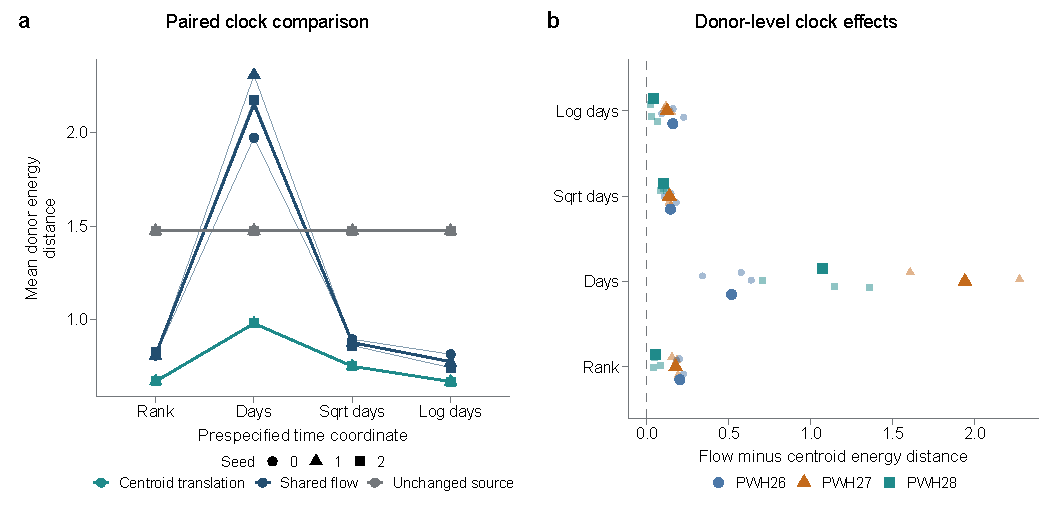
\includegraphics[width=\linewidth]{journal-figures/paper2_figure4_time_axes.pdf}
\caption{Paired time-coordinate sensitivity under global day-7 holdout in three healthy donors. Twelve fields cross four clocks with seeds 0, 1 and 2, each using 8,000 training steps and batch size 256. Initialization, endpoint draws and bridge random draws are paired across clocks within seed. Day 7 is excluded from fitting and scaling; 50 RK4 steps reach its exact transformed time, with identical evaluation rows and a 1,200-cell cap per donor. (a) Points are equal-donor means, shapes identify seeds, thin lines connect each seed and thick lines show seed means. Colors distinguish flow, centroid translation and unchanged source. Sqrt denotes square-root days; constant baselines overlap. (b) Large points show each donor's three-seed mean flow-minus-centroid error; small points retain the three seed-specific errors. Positive values favor the centroid and the dashed line marks no difference. Colors and shapes identify PWH26, PWH27 and PWH28 consistently across result figures. The centroid uses permitted day-1 and day-30 biopsies, so this remains retrospective interpolation. Clock connections are not biological trajectories; seed spread is not population uncertainty.}\label{fig:p2f4}\end{figure}

\begin{figure}[htbp]\centering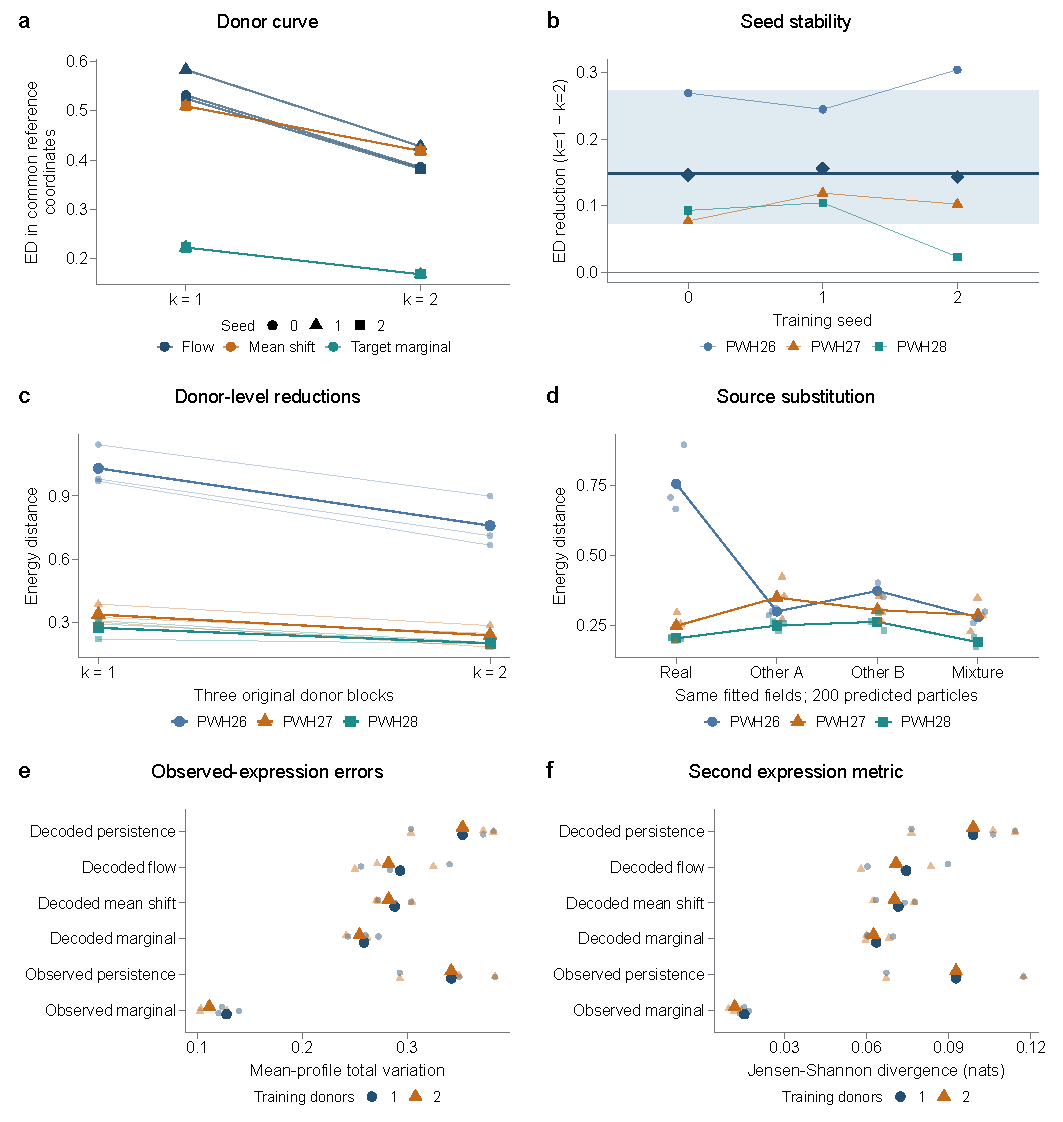
\includegraphics[width=\linewidth]{journal-figures/paper2_figure6_donor_curve_stability.pdf}
\caption{Donor count, source substitution and observed-expression restrictions. (a) Three-seed shared-flow curves alongside saved mean-displacement and exact target-marginal curves, in the same reference geometry and hierarchical donor weighting. (b) Macro seed reductions (navy diamonds; navy line, their mean), all nine donor/seed reductions and the saved descriptive three-block 95\% range; shading is not a seed-level interval. (c) Donor means with finer seed-resolved curves. (d) Real source, each alternative donor and their mixture under the saved 200-particle, 50-draw protocol; large points are donor means and smaller points are the three seed means. Other A/B are sorted alternatives within each fold. (e) Total variation against observed mean expression on 5,383 common genes. (f) Jensen--Shannon divergence for the same predictions. e/f distinguish decoded and directly observed predictors; large symbols are equal-donor macros and faint symbols are three donor means after seed/subset averaging, for each training size. Source mixing is not a donor-count experiment, and mean-expression errors are not full cellular-distribution validation. All panels reuse three donors; seeds, draws and overlapping folds add no biological replication.}\label{fig:p2f6}\end{figure}

\begin{figure}[htbp]\centering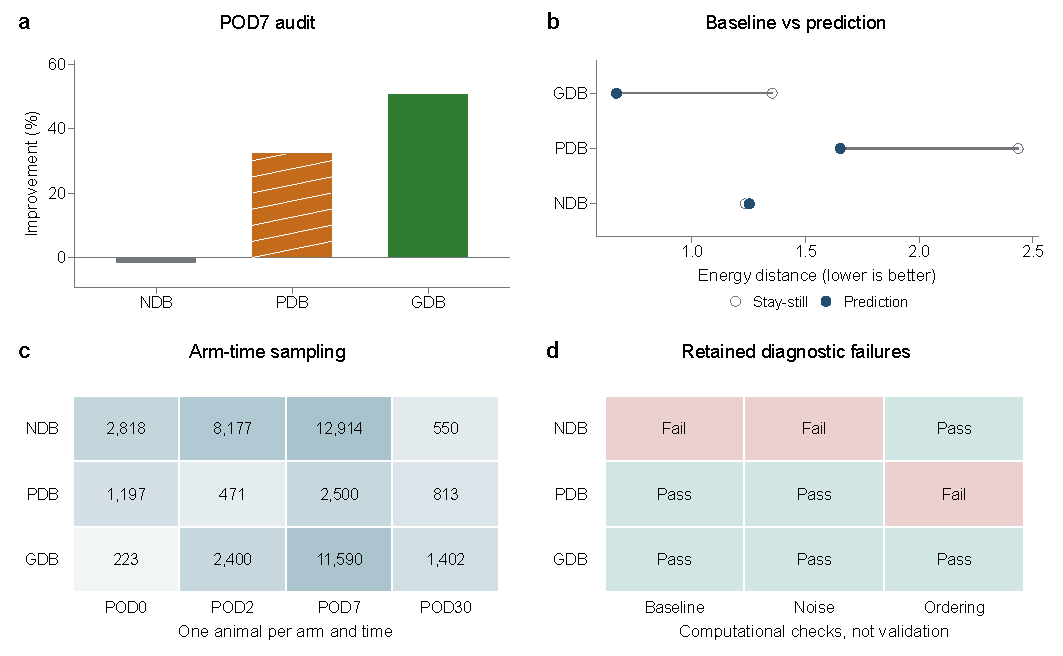
\includegraphics[width=\linewidth]{journal-figures/paper2_figure7_mouse_arms.pdf}
\caption{Mouse POD7 computational audit for NDB, PDB and GDB source arms. POD7 is excluded from fitting and scaling; fields trained at POD0, POD2 and POD30 predict from POD2. (a) Relative improvements −1.5\%, +32.1\% and +50.6\%; PDB hatching marks the failed endpoint-ordering check. (b) Connected unchanged-source and prediction errors on the absolute scale. (c) All 12 saved arm-time cell counts; color follows log-count and printed values are exact counts. Each entry has one animal, not multiple biological replicates. (d) Separate baseline, split-half noise and endpoint-ordering check outcomes, preserving every failure. Neither pass labels nor endpoint ordering establish biological trajectories. All arms cover 4,182/7,002 panel genes; no biological confidence intervals are available, and cells are not independent animals or clinical validation.}\label{fig:p2f7}\end{figure}

\FloatBarrier
\begingroup\setlength{\bibsep}{0pt}

\section*{Supplementary Methods}

\subsection{Source-bound symmetric repeated comparison}
An additional frozen-coordinate experiment compares persistence, mean translation, location--scale interpolation, permitted optimal-transport predictors, the training-target marginal and shared or source-conditioned fields under their respective missing-time and held-donor information sets. The two globally withheld times are days 1 and 7. Donor exclusion evaluates all three adjacent intervals; the day-1-to-day-7 interval remains separately identifiable. Source-replacement tasks exclude both the held donor and the substitute donor from fitting. Every neural field uses three seeds, 8,000 steps, three 256-unit hidden layers, a 32-dimensional time embedding, batches of 512 and 50 RK4 steps per interval. Optimizer steps do not imply equal wall time. Deterministic predictors use one fit seed, while stochastic target-marginal draws receive the same repeated evaluation contract.

Fifty draws select matched source and target particles within each task, donor, interval and draw, with at most 200 particles per distribution. Neural and moment-based predictors see the full permitted source before particle selection. The MMD bandwidth is frozen from training coordinates only and is not selected from predicted or evaluation-target cells. Energy distance, MMD, sliced Wasserstein, centroid and Bures discrepancies are retained. Every model and representation state is bound to its input and protocol, reloaded and replayed against the original training exclusions and evaluation identities before aggregation. Hash agreement alone is not accepted as scientific replay. A compact receipt binds the complete verified artifacts to the original input and current scientific implementation, allowing unchanged results to be summarized without copying checkpoints or repeating an already certified replay.

Comparisons average the log2 ratio of method error to a permitted baseline within a matched draw, then draws within fit and seeds within donor/task. Mean translation is the missing-time comparator and the equal-training-donor target marginal is the held-donor comparator. Negative ratios favor the listed method. Source-replacement ratios compare substituted and own-source errors from the same field and target draw. Undefined ratios remain explicit rather than being clamped. Ratios are descriptive, not an equal-compute test, a population ranking or cross-fold biological effect. All task intervals, unfavorable values, prediction warnings and transport marginal residuals are retained; repeated draws and seeds create no additional donors.

The original fields were fitted and evaluated on CUDA. Replay on the original CUDA backend retains all input, state, configuration, identity and score checks and the fixed prediction tolerance of absolute and relative $10^{-5}$. The separate CPU reintegration attempt retains its failed checks under that same tolerance; it is not reclassified as passing by the original-backend replay. This distinction qualifies the numerical portability of the saved predictions without changing a metric, model, source selection or target draw to improve its result.
\subsection{Coupling, coordinate and nested-selection follow-up}
The follow-up reuses the five primary human tasks, the original training exclusions, rank clock and matched evaluation draws. Independent-, exact-minibatch-OT- and entropic-bridge-coupled fields share three hidden layers of width 256, 512-cell batches, learning rate $10^{-3}$ and 8,000 optimizer steps; each has three seeds. Independent fields also receive a 40,000-step diagnostic. Full-source predictions are stored before scoring. The missing-time controls include a sampled exact endpoint-OT interpolant and its barycentric map. These endpoint controls receive the permitted later anchor; they are distinct from transferring a training-donor OT displacement to a held donor. Endpoint coupling defines a model path measure, not observed ancestry.

Five coordinate variants use the same task exclusions: standardized frozen encoder means, centered unscaled means, training-covariance whitening with eigenvalues floored at $10^{-6}$ times their mean, row-wise sum-zero encoder projection followed by training standardization, and 30 training-derived principal components of 2,000 training-selected variable genes. The sum-zero projection removes the common offset of the softmax coordinates; it does not create a new biological measurement. Independent and OT fields are fitted anew in each geometry. Ratios compare each field with its comparator inside the same geometry and donor; absolute distances across coordinate systems are not treated as interchangeable. Draw means are averaged within fit, seeds within donor, and then donors equally.

For held-donor selection, the outer donor is excluded from all inner fitting, representation preparation and scoring. Each inner fold trains on one of the other two donors and evaluates the remaining donor's day-1-to-day-7 distribution. The finite search uses 28 configurations: 18 independent-coupling, eight OT-coupling and two entropic-bridge settings. Widths, optimizer budgets and rates vary on unequal grids across families. Seed-0 matched-draw errors are averaged over the two inner folds to select a configuration. That configuration is then refitted on both permitted donors with three fresh seeds, giving nine outer refits. The outer targets enter only the final evaluation. This is selection within the existing cohort, not independent validation of the frozen discovery encoder.

An alpha scan changes the evaluation location of each fixed rank-trained field along its permitted source-to-anchor interval in increments of 0.05. Endpoint controls are evaluated at the same alpha. The held target supplies the displayed optimum, which is an oracle diagnostic and is never substituted for the declared prediction time. These scans do not retrain a field under a different clock.

\subsection{Source-distance, mixture and training-cell expression diagnostics}
Held-source energy and mean 15-neighbour distances are computed relative to the permitted training sources in each fold. Comparisons with distances between training donors describe geometry; no out-of-distribution threshold or calibrated rejection rule is fitted. Single-training-donor source-substitution fields and two-training-donor fields remain separate designs.

A further predictor mixes a transported source measure with the equally donor-weighted training target marginal:
\begin{equation}
\widehat P_w=w\widehat P_{\rm transport}+(1-w)\widehat P_{\rm marginal},\qquad w\in\{0,0.05,\ldots,1\}.\label{eq:p2shrinkage}
\end{equation}
Equation~\eqref{eq:p2shrinkage} mixes empirical measures, rather than averaging paired particles. Weighted V-statistic energy selects w in the two inner donor folds before outer evaluation. Mean translation and independent-coupling flow are assessed separately at all three adjacent intervals. The ratio is log2 of draw-averaged energies, followed by a seed mean; it is not the mean of per-draw log ratios used for the primary matched comparisons. Outer-target oracle weights are retained only as diagnostics.

For the held-donor expression diagnostic, every predicted coordinate is mapped to its 15 nearest permitted training cells and their mean per-cell gene-proportion profile on 5,383 common genes. This empirical decoder differs from the frozen topic decoder. Mean-profile total variation and Jensen--Shannon divergence are primary descriptions; fold-change rank correlations use 2,000 training-selected variable genes or a training-selected 50-gene signature. Metrics are averaged over seeds within donor and then over the three donors. Decoding observed held-target coordinates supplies a reconstruction reference, not a predictor or universal lower bound. The original missing-day-7 expression export covers only one donor and is not used as complete missing-time evidence here.

Input-backed reproduction rederives all 31 cached coordinate matrices and reloads all 354 original follow-up fields plus the nine new outer refits on CUDA at unchanged absolute and relative tolerances of $10^{-5}$. The new refits have input/code hashes fixed before fitting. The original fields receive a retrospective current-file manifest; their original training-time input hashes were not recorded, so successful saved-state replay does not establish identical retraining or historical fitting provenance. The saved alpha grids do not receive a new full-grid replay certificate. These limits are retained separately from the earlier failed CPU-portability gate.

\subsection{Data, representation and join integrity}
GSE241132 contains three healthy acute-wound donors, labelled PWH26, PWH27 and PWH28, with Skin, Wound1, Wound7 and Wound30 samples. Among 65,521 loaded cells, 58,823 joined the author metadata, and 12,259 author-annotated fibroblasts entered the temporal analysis. The fibroblast counts were 2,152, 1,012, 3,821 and 5,274 at the four times, respectively. Annotation is joined using sample identity and original cell-row identity before quality filtering; a filtered positional row number is not a valid substitute. Earlier exploratory outputs based on positional mismatching are invalid and contribute no results here.

The expression encoder is frozen from GSE165816; the human wound cohort was not used to refit it. It maps panel-normalized counts into a $q=15$ dimensional Gaussian-encoder mean $\mu$. Its training objective combines cross-entropy on cell proportions with a standard-Gaussian KL penalty of weight 0.01; it is not a Dirichlet model or an unmodified count-likelihood objective. Only 5,383 of 7,002 panel genes are covered in the human wound input (76.9\%); absent panel genes are zero-filled. The flow acts on $\mu\in\R^{15}$, not on simplex topic weights $\theta=\operatorname{softmax}(\mu)$. Softmax ignores a common additive coordinate offset, whereas Euclidean distance in $\mu$ need not. The frozen regularized encoder fixes a particular representation; the distance is not invariant to all representations producing the same simplex weights. Successful reconstruction is therefore conditional on this incomplete transferred panel and this coordinate system.

For training-cell set $\mathcal T$, scaling parameters are fitted coordinatewise on $\mathcal T$ only:
\begin{equation}
a_j=\frac1{|\mathcal T|}\sum_{i\in\mathcal T}\mu_{ij},\qquad
b_j=\left[|\mathcal T|^{-1}\sum_{i\in\mathcal T}(\mu_{ij}-a_j)^2\right]^{1/2},\qquad
z_{ij}=\frac{\mu_{ij}-a_j}{\widetilde b_j}.\label{eq:p2scale}
\end{equation}
In Equation~\eqref{eq:p2scale}, $\widetilde b_j=b_j$ for $b_j>0$ and $\widetilde b_j=1$ if $b_j=0$. The identical transformation is applied to source and target evaluation cells. The target is excluded from estimating $a_j,b_j$, and all cells of the held-out donor are excluded in donor transfer. Distances from different training folds are consequently expressed in their respective fold-standardized spaces.

\subsection{Two distinct held-out tasks}
Timepoint reconstruction. All Wound7 cells are withheld from fitting and scaling. Training segments are Skin$\rightarrow$Wound1 and Wound1$\rightarrow$Wound30 within each donor. The fitted field advances the observed Wound1 source to the specified Wound7 coordinate. The pooled analysis uses three donors. Three additional runs omit one donor and evaluate Wound7 in the remaining donors; these are sensitivity analyses, not predictions for the omitted donor.

Donor transfer. A donor is excluded entirely from fitting and scaling; all four time points in the other two donors are retained. Adjacent within-donor segments Skin$\rightarrow$Wound1, Wound1$\rightarrow$Wound7 and Wound7$\rightarrow$Wound30 are used. The held donor's Wound1 cells initialize prediction, while their Wound7 cells are used for evaluation only. Because Wound7 is observed in training donors, this task does not test reconstruction of a globally unobserved time point. The method benchmark and donor-count experiment use this latter design. Supplementary Table~S14 lists the exclusions and settings. A target-marginal baseline therefore uses the observed Wound7 distributions of training donors, which are unavailable in global Wound7 holdout.

\subsection{Time coordinates and conditional flow matching}
Let $P_t^{(d)}$ denote the empirical distribution of standardized fibroblast coordinates for donor $d$ at day $t$. Write $s=g(t)$ for transformed time. Rank time assigns $(0,1/3,2/3,1)$ to days $(0,1,7,30)$, and the other tested transforms are
\begin{equation}
g_{\rm days}(t)=t/30,\qquad
g_{\rm sqrt}(t)=\sqrt{t/30},\qquad
g_{\rm log}(t)=\log(1+t)/\log31.\label{eq:p2times}
\end{equation}
Equation~\eqref{eq:p2times} defines the three day-based alternatives to rank time. For one training donor and segment $(s_a,s_b)$, endpoints are sampled independently from the source and target cells of that donor. Thus the training coupling is the empirical product $\pi_{d,ab}=P_{t_a}^{(d)}\otimes P_{t_b}^{(d)}$. It is not an optimal-transport coupling and does not pair the same biological cell across times. With $\lambda\sim U(0,1)$,
\begin{equation}
z_\lambda=(1-\lambda)z_a+\lambda z_b,\quad
s_\lambda=(1-\lambda)s_a+\lambda s_b,\quad
u_{ab}=\frac{z_b-z_a}{s_b-s_a}.\label{eq:p2bridge}
\end{equation}
Equation~\eqref{eq:p2bridge} defines the interpolated state, time and target velocity. Let $\mathcal A$ be the list of available donor--segment pairs and $h_{ab}=s_b-s_a>0$. The implementation cycles through this list, so pair counts differ by at most one batch over 8,000 steps. Its ideal uniformly weighted objective is
\begin{equation}
\mathcal L_{\rm CFM}(\phi)=\frac1{|\mathcal A|}\sum_{(d,a,b)\in\mathcal A}\frac1{h_{ab}}
\int_{s_a}^{s_b}\E_{\pi_{d,ab}}\!\left[\frac1q\|v_\phi(z_{(s-s_a)/h_{ab}},s)-u_{ab}\|_2^2\right]ds.\label{eq:p2cfm}
\end{equation}
Equation~\eqref{eq:p2cfm} averages squared error over batch examples and coordinates. The factor $1/h_{ab}$ follows from sampling $\lambda$ uniformly on each segment; dividing $z_b-z_a$ by $h_{ab}$ gives velocity per unit transformed time. Donors therefore receive approximately equal training weight within a segment, regardless of their cell yields. Scaling and the original pooled evaluation instead weight retained cells equally. These measures need not coincide. Equations~\eqref{eq:p2bridge}--\eqref{eq:p2cfm} implement conditional flow matching with a product coupling; they do not solve the Benamou--Brenier minimum-kinetic-energy problem. On a single training segment, the marginal law of an exact solution is the independent bridge in Equation~\eqref{eq:p2interpolation}: the distribution of convex combinations of independently drawn endpoints. A field shared across segments and donors, or stopped at finite capacity, need not realize that law. A lower error than the bridge is therefore not evidence that the training objective targets displacement interpolation.

A pure change of time coordinate for an already specified physical-time field $v_t$ would require
\begin{equation}
v_s(z,s)=\frac{v_t(z,g^{-1}(s))}{g'(g^{-1}(s))},\qquad 0<g'(t)<\infty.\label{eq:p2clock}
\end{equation}
Equation~\eqref{eq:p2clock} is the chain rule, not the procedure used in the time-axis experiment. Each tested axis instead defines new straight bridges, new segment widths and a separately fitted field with the same optimization budget. The original axis comparison used one network seed while endpoint-sampling random draws advanced across axes, so clock and training variation were not independently isolated. A short segment increases target-velocity magnitude and alters the loss density in time. Performance differences consequently combine modeling and optimization effects; they cannot isolate a biological clock or prove that interval compression caused an observed failure.

A subsequent paired-clock audit fixed seeds 0, 1 and 2 across all four transforms, giving 12 fields at the same 8,000-step, batch-256 budget. Within each seed, network initialization, endpoint indices and Torch interpolation draws are identical across clocks and checked by their recorded fingerprints. Day-7 observations are excluded globally from fitting and from the common training scaler. Each field advances the same day-1 cells to the exact transformed day-7 time using 50 RK4 steps, with a separate 200-step refinement. Identical source and target row selections, capped at 1,200 per donor, are reused across clocks and seeds. The centroid comparator shifts each source by the transformed-time fraction of that donor's observed day-1-to-day-30 mean displacement; neither predictor uses day-7 expression. Errors are averaged equally over donors and then seeds. Checkpoints are independently reloaded and reintegrated on CPU before scores are accepted. This repeated comparison addresses the random-stream and nearest-grid-point defects of the historical clock experiment, but it does not add donors, select a clock on independent data or pair the separate conditioned-field and transport method benchmark.

Following the neural ordinary-differential-equation formulation, predictions solve an initial-value problem and push forward the empirical source measure:
\begin{equation}
\frac{dz}{ds}=v_\phi(z,s),\qquad z(s_a)=z_a,\qquad
\widehat P_{s_b}=(\Phi^\phi_{s_a\rightarrow s_b})_\#\widehat P_{s_a}.\label{eq:p2ode}
\end{equation}
Equation~\eqref{eq:p2ode} defines prediction from the observed source distribution. The network uses two 128-unit SiLU hidden layers and a 32-dimensional sinusoidal time embedding. Training uses Adam with learning rate $10^{-3}$, 8,000 steps and batches of 256. Direct target predictions use 50 fixed fourth-order Runge--Kutta steps. The time-axis diagnostic instead uses 60 steps over the full Wound1-to-Wound30 segment and reads the grid point nearest the transformed Wound7 coordinate; it does not select the grid point with the lowest target distance. A separate fixed-field resolution comparison is described below; finite-step agreement does not prove convergence to an exact solution.

\subsection{What distributional success does and does not identify}
At the unrestricted square-integrable minimizer, the field is $v^*(z,s)=\E[u_{ab}\mid z_\lambda=z,s_\lambda=s]$ under the training sampling measure. The standard squared-error decomposition leaves an irreducible conditional velocity variance plus the error in approximating $v^*$. Within a common observed segment, let $P_s$ be the donor-balanced mixture of the product-coupling paths. For a smooth compactly supported test function $f$,
\begin{align}
\frac{d}{ds}\int f(z)\,dP_s(z)&=\E[\nabla f(z_s)^{\mathsf T}u_{ab}]
=\int\nabla f(z)^{\mathsf T}v^*(z,s)\,dP_s(z),\notag\\
\partial_s p_s+\nabla\!\cdot(p_sv^*)&=0\quad\text{when a density exists}.\label{eq:p2continuity}
\end{align}
Equation~\eqref{eq:p2continuity} states probability conservation first in weak form, which does not presume that empirical atomic measures have a density. Identifying its solution with a unique deterministic ODE push-forward requires additional regularity; the weak identity alone supplies no such guarantee for empirical endpoints. Finite neural fitting and integration introduce further approximation. Moreover, Wound7 is not an endpoint in the globally withheld-time training path, and a cell-weighted source need not equal its donor-balanced source. The flow-matching identity therefore does not guarantee either the held-out biological distribution or the originally pooled evaluation score.

Normalized probability transport does not identify cell proliferation, death or ancestry. Recovery of underlying dynamics from marginal observations requires assumptions beyond matching those observations. The present analysis does not verify the diffusion and sampling conditions of trajectory-identification theory. With four measurement times, the values of $g$ between observations remain analysis choices.

\subsection{Distance estimand, finite-sample statistic and thresholds}
For independent $X,X'\sim P$ and $Y,Y'\sim Q$ with finite first moments, define energy distance without the optional square root:
\begin{equation}
D_E(P,Q)=2\E\|X-Y\|_2-\E\|X-X'\|_2-\E\|Y-Y'\|_2.\label{eq:p2ed}
\end{equation}
In Euclidean space, Equation~\eqref{eq:p2ed} is nonnegative and zero exactly when $P=Q$. The implementation uses the V-statistic, including diagonal zero distances:
\begin{align}
\widehat D_E(P_m,Q_n)={}&\frac{2}{mn}\sum_{i=1}^{m}\sum_{j=1}^{n}\|x_i-y_j\|_2
-\frac1{m^2}\sum_{i=1}^{m}\sum_{i'=1}^{m}\|x_i-x_{i'}\|_2\notag\\[-2pt]
&-\frac1{n^2}\sum_{j=1}^{n}\sum_{j'=1}^{n}\|y_j-y_{j'}\|_2.\label{eq:p2edv}
\end{align}
Equation~\eqref{eq:p2edv} is the exact distance between the two empirical measures, not an unbiased U-statistic for the population distance. For baseline $B=\widehat D_E(P_{\rm source},P_{\rm target})>0$ and predicted distance $D$, gain and relative improvement are
\begin{equation}
G=B-D,\qquad I=G/B=1-D/B.\label{eq:p2improvement}
\end{equation}
Equation~\eqref{eq:p2improvement} defines the absolute gain and the fraction reported as a percentage. Stay-still means $P_{\rm prediction}=P_{\rm source}$. Seeded subsampling caps the quadratic distance calculation at 1,500 cells per distribution for initial timepoint reconstruction and at 1,200 for donor transfer, the common method benchmark and the donor-count analyses. Counts, caps and per-fold values accompany each comparison; independently run analyses need not have identical stochastic point estimates.

Scoring an equal mixture is not equivalent to averaging its component scores. For $M=(P_1+P_2)/2$, expansion of Equation~\eqref{eq:p2ed} gives
\begin{equation}
\frac{D_E(P_1,Q)+D_E(P_2,Q)}{2}-D_E(M,Q)=\frac14D_E(P_1,P_2).\label{eq:p2mixture}
\end{equation}
Equation~\eqref{eq:p2mixture} holds for the unsquared-root discrepancy and exact weighted empirical measures in fixed coordinates. Its right-hand side contains no test target $Q$. Thus, the reduction from averaging two single-donor target-marginal errors to scoring their mixture is a mathematical consequence of the difference between those training distributions, not independent evidence that the second donor contributes target-specific information. It does not equate a jointly fitted two-donor neural field with a mixture of two separately fitted fields.

The target is split once into seeded disjoint halves, defining $N=\widehat D_E(P_{\rm target,1},P_{\rm target,2})$. The initial timepoint report asks only whether $G>0$, while the time-axis, donor-transfer, method and donor-count comparisons use $G>N$. The latter is a sampling-scale heuristic, not a significance test with known type-I error, a repeated-resampling interval, or an error bound. A gain larger than this within-target sampling scale does not separate methods that all improve on an unchanged source. Selecting the best position on a path using target distances is retrospective; the preassigned Wound7 coordinate supplies the held-out result, and the full scan is a diagnostic rather than a tuned clinical predictor.

\subsection{Donor context and the non-neural predictors}
For a source sample, context concatenates the coordinatewise mean and population standard deviation (divisor $n$), $c_d=(\bar z_d,\operatorname{sd}(z_d))\in\R^{2q}$. The conditioned field uses this context from the training segment's source. Independently for each training example $i$,
\begin{equation}
B_i\sim\operatorname{Bernoulli}(0.8),\qquad \widetilde c_i=B_i c_d,\qquad
\mathcal L_{\rm context}=\E\!\left[q^{-1}\|v_\phi(z_i,s_i,\widetilde c_i)-u_{ab,i}\|_2^2\right].\label{eq:p2context}
\end{equation}
Equation~\eqref{eq:p2context} masks the entire context vector per example, rather than masking an entire batch or individual context coordinates. At test time there is no mask, and the held donor's source alone supplies $c_d$. Training with zero context does not guarantee agreement with a separately trained shared field, bounded extrapolation or successful donor transfer. Both neural fields use the same donor-segment schedule and endpoint-sampling rule, although successive pseudorandom draws need not be identical. The original five-predictor comparison used one seed and did not pair endpoint random draws across model classes; its method ordering is conditional on those fits. Six training-donor evaluations are reported separately from the three held-out-donor folds.

Let $\delta_d=\bar z_{d,7}-\bar z_{d,1}$ for a training donor. Mean displacement predicts $z+\overline\delta$; nearest-donor displacement predicts $z+\delta_{d^*}$, where $d^*$ maximizes cosine similarity between the source contexts. These are translations, not fitted neural fields. The entropic transport baseline uses pooled training-source and training-target cells, uniform empirical marginals $a,b$, and normalized squared Euclidean cost $C$:
\begin{equation}
\Gamma_\varepsilon=\arg\min_{\Gamma\geq0,\,\Gamma\mathbf1=a,\,\Gamma^{\mathsf T}\mathbf1=b}
\left\{\langle C,\Gamma\rangle+\varepsilon\sum_{ij}\Gamma_{ij}(\log\Gamma_{ij}-1)\right\},\quad\varepsilon=0.05.\label{eq:p2ot}
\end{equation}
Equation~\eqref{eq:p2ot} defines the entropic transport plan fitted to the training endpoints. Specifically, $C_{ij}=\|z_i-z_j\|_2^2/\max_{kl}\|z_k-z_l\|_2^2$, so the regularization value is relative to the largest sampled training cost. The POT implementation caps Sinkhorn iteration at 2,000 steps, with at most 1,500 cells per endpoint. Row-normalized barycentres define training-source displacements; each held-out source cell receives the average displacement of its 15 nearest training-source neighbours. This is an out-of-sample displacement extension of a transport plan, not transport fitted to the held target. A finite iteration budget alone does not certify exact marginal feasibility or optimality.

\subsection{Separate finite-budget paired diagnostics}
An additional saved diagnostic excludes each of PWH26, PWH27 and PWH28, fits representation preprocessing only in the other two donors and evaluates the three adjacent intervals 0$\rightarrow$1, 1$\rightarrow$7 and 7$\rightarrow$30. Every interval starts from its observed source, not an autonomous rollout from day 0. Training-side selection of 200 variable genes followed by 15-dimensional PCA defines a different representation from the frozen neural coordinates used in the primary analyses. PCA scaling is fold-specific, so distances are interpreted within donor rather than pooled across folds as a biological effect.

Independent-endpoint, minibatch optimal-transport, entropic-bridge and source-context-conditioned flows each use two seeds at 120 and 600 steps, giving 48 fits. These diagnostic fields have two 64-unit hidden layers, a 16-dimensional time embedding and batches of 64; they are not architecture- or budget-matched reproductions of the primary 8,000-step fields. Persistence, mean shift, location--scale and a fixed seed-0 equal-training-donor target draw add 12 baseline jobs, producing 180 dependent prediction pairs in total. Energy V-distance is capped at 200 cells per distribution. Within each donor and budget, errors average the three intervals and two flow seeds equally. Equal optimizer steps are not equal wall time, and one baseline draw does not establish symmetric stochastic stability. Adaptive MMD uses prediction-plus-target bandwidth and is retained only as a diagnostic, not a cross-method ranking. All entropic-coupling residuals and failed marginal-tolerance screens are retained. Saved predictions were verified without refitting; the historical diagnostic does not provide reloadable fields (Supplementary Table~S41 and~S42).

Complete saved within-donor method and budget means are provided in Supplementary Table~S42.

\subsection{Target-marginal comparison and a common donor-count scoring scale}
The added target-marginal predictor assigns equal mass to each permitted training donor's observed Wound7 distribution. It uses no expression values from the held donor's Wound1 source. For comparison with the historical method benchmark, 50 without-replacement draws match its 255, 497 and 260 predicted particles in the three held-donor folds, using the identical seed-0 target indices and original training-only standardization. Particle counts are balanced between the two training donors, and each donor receives exactly one half of total weight under Equation~\eqref{eq:p2weighted}. Uniform-particle scores are also retained to quantify the negligible weight difference from an odd particle count. The historical field was not saved with its per-cell predictions; its reported error is therefore a fixed reference, not a field reevaluated on new target draws. The 50 draws quantify target-marginal sampling variation in the same three donors (Supplementary Table~S35).

A separate controlled rerun fits all 27 shared fields defined by three seeds, three held donors and two single-donor or one two-donor training configurations. Each fit resets both endpoint-sampling and network random generators, retains the original architecture and optimization budget, and saves its predictions and training scaler. Training normalization continues to use only the selected training subset. For evaluation, predictions are first returned to the frozen encoder coordinates, then transformed using one reference scaler estimated from both available non-held donors across all times. The reference is fixed within held donor across k and seed, and is used only for scoring: it is not supplied to a single-donor fit. Identical observed source and target samples are scored in this common geometry. This separates adding training information from changing the distance metric. Mean displacement and empirical target-marginal predictions use only the selected training donors and are scored under the same reference. The earlier curve subtracted distances from different training-subset scalers and is superseded for absolute k comparisons.

A retrospective source-replacement audit reuses the nine saved two-training-donor fields (three held donors, seeds 0--2) without refitting. Each field first predicts from the excluded donor's actual Wound1 cells, then from an equal-donor mixture of the two permitted training donors' Wound1 cells. Fifty draws sample without replacement at exactly the held-source particle count (255, 497 or 260), and the same field transports both sources for the same Wound1-to-Wound7 interval. The substituted sources have half their probability mass from each training donor; the actual source is uniformly weighted within its single donor. Predictions are returned through the saved training scaler into the same held-donor reference coordinates and compared with identical saved Wound7 target cells. The already calculated, equally weighted training-donor Wound7 marginal uses the same target indices and particle count but separate draw samples; draw numbers across these two controls do not form paired biological measurements. We average draws within field, then seeds within held donor, then the three donors equally. Source substitution tests sensitivity of these fixed fields to their input distribution; it cannot identify individual cell fates, establish a donor-population effect or independently validate the choice of model (Supplementary Table~S36).

A further saved-prediction audit separates individual source substitutions from mixed substitutions. It first verifies Equation~\eqref{eq:p2mixture} using the complete permitted training-Wound7 distributions in each fixed reference. It then scores 200 predicted particles from the real source, 200 from each individual permitted training donor's source, and a 200-particle mixture containing 100 from each training donor. Fifty without-replacement draws share the original held-target indices and reuse source indices across all three fitted seeds. The mixture uses prefixes of each individual draw, with exact half donor masses. A second identity check compares the mixture with its actual 100-particle components; the difference between the 200-particle individual scores and the 200-total mixture is not substituted into that identity. Nine saved checkpoints are reintegrated on CPU as a consistency check, without fitting. Draw means are averaged within seed, then seeds within held donor, then donors equally. This is an additional fixed-field sensitivity estimand: it changes source identity, in-training versus held-source status and, for the mixture, diversity, while adding no independent donors (Supplementary Table~S38).

\subsection{Donor-count estimand and dependence-aware summaries}
For each held donor $d$ and seed $r\in\{0,1,2\}$, let $D_{1,d,r}$ average the errors from the two possible single-training-donor choices, and let $D_{2,d,r}$ be the error with both available training donors. Equal weighting then gives
\begin{equation}
R_k=\frac1{3\cdot3}\sum_{d=1}^{3}\sum_{r=0}^{2}D_{k,d,r},\qquad
\Delta_d=\frac13\sum_{r=0}^{2}(D_{1,d,r}-D_{2,d,r}),\qquad
\overline\Delta=\frac13\sum_d\Delta_d.\label{eq:p2curve}
\end{equation}
Equation~\eqref{eq:p2curve} defines the seed-averaged estimand and donor-block differences. All distances in Equation~\eqref{eq:p2curve} use the common reference within held donor. The plotted main curve uses seed 0, with other seeds shown separately. The 4,000-draw percentile interval resamples the three $\Delta_d$ blocks after averaging seeds. With three blocks, its central 95\% percentile endpoints are the minimum and maximum of those three reductions, so the interval is not a calibrated population quantile. Overlapping training donors still induce dependence between held-out errors, and the interval remains a descriptive three-block summary. Seeds and alternative training subsets are not additional biological replicates. Configuration-specific ranges quantify stochastic instability. Two values of $k$ cannot identify a plateau, a functional learning-curve model or a required number of donors.

\subsection{Geometry and mouse computation}
Donor displacement alignment is $\cos(\delta_d,\delta_e)=\delta_d^{\mathsf T}\delta_e/(\|\delta_d\|\|\delta_e\|)$. The time-versus-donor contrast compares 18 within-donor temporal distances with 12 between-donor same-time distances. Pair-distance bootstrap intervals are descriptive because pairs share donors. The geometric screen used for endpoints $a,b$ and held time $h$ is
\begin{equation}
J=\ind\{\widehat D_E(P_a,P_b)\geq\max[\widehat D_E(P_a,P_h),\widehat D_E(P_h,P_b)]\}.\label{eq:p2geometry}
\end{equation}
Equation~\eqref{eq:p2geometry} is a distance-ordering diagnostic. It does not imply equality in a triangle inequality, identify a geodesic, or establish that a target lies on a unique direct path. We report it as such rather than as proof of interpolability.

GSE326622 \citep{berryman2026mechanotransduction} is evaluated separately for the source-labelled NDB, PDB and GDB mouse arms. POD7 is excluded from fitting and scaling; POD0, POD2 and POD30 provide the training time points, with POD2 supplying the prediction source. Each mouse fit uses rank time, 6,000 optimization steps and batches of 256. The human panel's mouse-symbol mapping covers 4,182 of 7,002 genes (59.7\%) in each arm, and each arm has one animal per time point. Animal identity and time are therefore confounded. The three arm computations assess protocol behaviour and representation transfer; cell numbers do not supply independent animals or cross-species clinical validation.

\subsection{External cross-sectional mouse series}
GSE186527 supplies a second mouse series \citep{mascharak2022multiomic}. Nine pooled libraries each contain cells from five mice, sorted into a lineage-negative fibroblast-enriched gate (Lin$-$) and a lineage-positive gate of the remaining cells (Lin+) and labelled with ten hashtag oligonucleotides (HTOs); the authors' dictionary maps every library and HTO to a day, treatment arm, mouse and gate. Each animal is sampled once, so a mouse is nested within an arm and day and no animal or cell is observed twice. The protocol, admission floors, methods and metrics were frozen before any expression-level analysis. HTO counts were located by feature type and classified with a fixed rule (top count at least 20 and at least five times the second); a looser and a stricter rule report sensitivity. Day and arm were taken from the library for the six libraries with usable HTO counts, and mouse and gate from the HTO. The three unwounded and POD2 libraries contain no HTO counts in any cell and are excluded. As for the GSE326622 arms, a treatment arm plays the role of an individual; a population is the cells of one arm, day and gate, and must contain at least 50 cells from at least two mice. Mouse 5 is excluded from the Lin+ gate because the dictionary labels both of its tags Lin+; no label is corrected. Leave-one-individual-out and donor-count tasks do not apply because no animal is sampled twice.

The missing-time task withholds POD14, with POD7 as source and POD30 as a later anchor, so it is a retrospective interpolation. The representation is a 30-component PCA of 2,000 variable genes fitted without POD14 cells of the analysed gate. The nine methods permitted by the missing-time information set (stay-still, mean shift, location--scale, quantile map, optimal-transport (OT) displacement, Gaussian geodesic, and flow matching with independent, OT and Schr\"odinger-bridge couplings at 8,000 steps and three seeds) are scored with the squared energy statistic against all held cells and, separately, against each held mouse. Location--scale is the declared comparator, a log-days clock is run for two methods as sensitivity, and results are descriptive: arms, gates and mice are not pooled into an inferential unit.

\subsection{Numerical-resolution and evaluation-sampling sensitivity}
The saved human expression coordinates and annotations supply a separate seed-0 pooled fit using the stated training exclusions, 8,000 optimization steps and batch size 256. The fitted field is then fixed. Predictions integrate the same 1,012 day-1 cells with 25, 50, 100 and 200 RK4 steps to the prespecified rank-time day-7 coordinate. Distance calculations use one fixed set of 1,500 day-7 cells and double-precision pairwise distances. Root-mean-square coordinate discrepancies are measured relative to the 200-step result (Supplementary Table~S27).

Evaluation sensitivity fixes the 50-step prediction and varies only cell subsampling. At each count of 250, 500 and 1,000 cells per distribution, 50 seeded draws without replacement use common source and target indices for predicted and unchanged-source distances. Each draw additionally samples two disjoint target subsets of that size for the reference distance. We report median improvement, the central 95\% range across draws and the count exceeding the reference (Supplementary Table~S28). These are conditional Monte Carlo summaries. They neither refit the field per draw nor estimate uncertainty across new donors.

\subsection{Evaluation weights and mathematical verification}
A further analysis fixes that same 50-step field prediction, retains all 1,012 source cells and 3,821 target cells, and changes only empirical weights. For nonnegative unit-sum weights $a,b$, the exact weighted empirical distance is
\begin{align}
\widehat D_{E,a,b}={}&2\sum_{i,j}a_i b_j\|x_i-y_j\|_2
-\sum_{i,i'}a_i a_{i'}\|x_i-x_{i'}\|_2\notag\\
&-\sum_{j,j'}b_jb_{j'}\|y_j-y_{j'}\|_2.\label{eq:p2weighted}
\end{align}
Equation~\eqref{eq:p2weighted} uses equal cell weights for the original pooled estimand. Equal donor mass instead assigns each cell from donor $d$ weight $1/(3n_d)$, separately at source and target; predicted cells retain their source weights. We also evaluate each donor using this same pooled time-holdout field. Those rows are not new donor-transfer fits. This analysis changes neither scaling nor training weights, and it supplies no additional donor-level uncertainty estimate (Supplementary Table~S29).

Executable checks compare interval-scaled flow loss with an analytic translation, the context mask with a prescribed per-example draw, RK4 with translation and exponential ODE solutions, and weighted energy distance with explicitly replicated empirical samples. Invalid time spans, endpoint shapes and dropout probabilities are rejected before training. These checks verify mathematical implementation properties; they do not substitute for held-out biological evaluation. Numerical-order claims follow the usual smoothness assumptions for RK4.

\subsection{Observed-cell geometry and raw expression context}
The tissue drawing is a conceptual account of the sampled material, not a histological observation. The expression display uses a fresh raw-matrix reconstruction with author annotations joined by sample and barcode under the verified row contract. Retained fibroblast sample, donor and time ordering must match all 12,259 saved temporal coordinates. Twelve specified matrix, inflammatory and contractile genes are summarized separately in each of the 12 biopsies. Counts are pooled within the biopsy, divided by its total fibroblast count-library size, scaled to 10,000 and transformed by $\log(1+x)$. Each gene is then scaled between its minimum and maximum across biopsies for display. No expression-difference test, inferred spatial position or cell lineage is obtained from this descriptive heat map.

Principal component analysis is fitted on the 8,438 standardized cells available in the global day-7 training set. Every displayed time and model prediction is projected onto that fixed basis. A seed-17 uniform subset of 2,000 observed fibroblasts supplies both time-colored and donor-colored panels. Thirty-six uniformly selected day-1 source cells supply the displayed paths, sampled at 11 evenly spaced model times under the seed-0 field. Intermediate coordinates are obtained by 50-step RK4 integration from the same source to each requested time. The projection can omit relevant state variation; all prediction errors continue to use the full 15-dimensional coordinates. Arrows indicate numerical evolution under the fitted field and do not identify the fate of observed cells.

\subsection{Global missing-time baselines and a second interpolation target}
A separate retrospective comparison fixes two global exclusions, day 7 and day 1. The original rank coordinates remain $0,1/3,2/3,1$ even after a time is excluded. For withheld day 7, training segments connect day 0 to day 1 and day 1 to day 30; for withheld day 1, they connect day 0 to day 7 and day 7 to day 30. Standardization excludes every held-time cell. All three donors remain in the training cohort, and the original within-donor product endpoint sampling, network, learning rate, 8,000 optimization steps and batch size 256 are retained. Three independent fits use seeds 0, 1 and 2. The extension does not retune the clock or use held-time error to choose an integration endpoint.

Let $a<h<b$ be the source, held and next available times on this rank axis, and let $\alpha=(h-a)/(b-a)$. For a source cell $z_i$ from donor $d$, the two explicit interpolation controls are
\begin{equation}
\widehat z_i^{\rm mean}=z_i+\alpha(\bar z_{d,b}-\bar z_{d,a}),\qquad
\widehat z_i^{\rm bridge}=(1-\alpha)z_i+\alpha Z_{d,b},\quad
Z_{d,b}\sim\widehat P_{d,b}.\label{eq:p2interpolation}
\end{equation}
Equation~\eqref{eq:p2interpolation} translates the entire source distribution by its donor's interpolated mean displacement or independently samples an anchor cell for each source cell. Anchor draws use replacement and seeds 0, 1 and 2; the mean translation is deterministic. Both tasks have $\alpha=1/2$. Source and anchor biopsies are available in training, while the target biopsy is withheld. These baselines do not solve an optimal-transport coupling. The bridge can contract or otherwise alter dispersion, whereas translation preserves the source's centered distribution. Neither construction is a measured cell trajectory.

To prevent donors with more recovered cells from dominating this comparison, compute the empirical energy distance separately for each donor using all its target cells and all source-derived predictions, then use
\begin{equation}
R_{m,r,h}=\frac13\sum_{d=1}^{3}\widehat D_E(\widehat P_{m,r,d,h},\widehat P_{d,h}),\qquad
I_{m,r,h}=1-\frac{R_{m,r,h}}{R_{\rm unchanged,h}}.\label{eq:p2macroerror}
\end{equation}
Equation~\eqref{eq:p2macroerror} defines the donor-averaged error and corresponding improvement; it is not a pooled distance with equal donor mass because it omits cross-donor distance terms. Distances use double precision in all 15 training-standardized coordinates, with no cell cap. We retain every donor and seed, average seeds only after each donor comparison, and report seed ranges without interpreting them as biological confidence intervals. The source and anchor differ between tasks, so their absolute errors are conditional on different training scalers and targets. Access to each donor's later anchor makes this retrospective reconstruction, not prospective source-only prognosis.

\subsection{Observable mean-expression audit of saved donor-transfer predictions}
The expression-space audit reuses all 27 saved donor-count fits without retraining. Raw count rows are joined by archive, barcode and author label to all 12,259 fibroblast encoder means; re-encoding checks this alignment. The primary feature set is every frozen-panel gene present in all twelve assay feature catalogues: 5,383 of 7,002 genes. It uses no expression-variance or favorable-performance filter, although use of the evaluation assay catalogues means this is not an assay-blind external design. The remaining 1,619 genes are unmeasured, not observed zeros. Protocol, feature list, training-derived signatures and input/code fingerprints are fixed before the new predictive scores are computed.

Each predicted standardized coordinate is returned through its fit-specific training scaler to $\mu$. Its gene-proportion vector is $\operatorname{softmax}(\mu)\beta$. The vector is restricted to the common panel and normalized per particle before averaging; decoder rows are not separately renormalized before topic mixing. Observed count rows undergo the same common-panel normalization before equal-cell averaging, rather than pooling library counts. A zero common-panel total fails the analysis instead of silently dropping a cell. The primary target uses exactly the saved held-day-7 evaluation rows; all held-day-7 cells form a prespecified overlapping sensitivity, not an independent replication.

Comparators use the same permitted training-donor subsets and held-source identities: decoded persistence, saved mean displacement, and the equally donor-weighted training-day-7 marginal. Directly observed persistence and training-target marginals are separately labelled controls. Training marginals are legitimate here because this is donor transfer, not global timepoint holdout. Total variation between the mean gene profiles is primary; Jensen--Shannon divergence with natural logarithms and gene-wise root mean square error are secondary. Seed means are averaged within training subset, subsets within held donor, and the three held donors equally. No cell bootstrap, significance test or biological interval is supplied. Secondary signed gene sets use the 25 most increased and 25 most decreased genes in the permitted training donors only; they are descriptive expression signatures, not validated pathways. Decoding the observed target cells supplies a separately reported reconstruction reference and missing-panel mass; it is not a forecast, true expression or a mathematical lower error bound. Mean-profile agreement does not imply absolute-count prediction, complete distributional fidelity or individual cell transitions.

\subsection{Endpoint dispersion and distribution-shape controls}
A further deterministic baseline asks whether endpoint dispersion helps beyond translating the mean. For each donor and coordinate $j$, let $s_{a,j}$ and $s_{b,j}$ be empirical standard deviations at the allowed source and anchor, using denominator $n$. The location--scale predictor is
\begin{equation}
\widehat z_{ij}^{\rm scale}=(1-\alpha)\bar z_{a,j}+\alpha\bar z_{b,j}
+\frac{(1-\alpha)s_{a,j}+\alpha s_{b,j}}{s_{a,j}}(z_{ij}-\bar z_{a,j}).\label{eq:p2locationscale}
\end{equation}
Equation~\eqref{eq:p2locationscale} preserves source standardized residuals and interpolates coordinate means and standard deviations at the same fixed $\alpha=1/2$. A source standard deviation at most $10^{-8}$ gives zero residual contribution in that coordinate. This rule uses neither target cells nor outcome-based tuning and does not interpolate the full covariance or estimate an optimal coupling.

For each of the five predictors, donor, held time and existing fit seed, we calculate full-cell energy distance, Euclidean distance between predicted and target centroids, the ratio of total coordinate variances, and energy distance after separately centering each distribution by its own mean (Supplementary Table~S33). Centering uses the target mean only during evaluation. The centered distance is a separate location-invariant shape diagnostic; it is not an additive term in a decomposition of the original energy distance. Donor summaries have equal weight, with seeds averaged within donor.

A matched cell-count evaluation uses 50 draws of 200 source and 200 target cells per donor and held time, without replacement, with random seed 29. The same indices select source-derived predictions and observed targets for all methods and training seeds in a draw. Averaging first within donor and then equally over the three donors yields paired flow-minus-comparator differences (Supplementary Table~S34). Ranges across draws describe sensitivity to the observed cells, not independent donor replication, confidence intervals or a significance test. Previously reported full-cell baseline errors must be reproduced before the additional diagnostics are accepted.



OpenAI Codex (OpenAI) assisted with code development, execution and checking of computational analyses, suggestions for analytical and methodological checks, manuscript drafting and restructuring, extensive language editing, and LaTeX and figure preparation. Reported numerical results were checked against saved outputs, and scripts and document builds were verified using the procedures described in this article and its Supplementary Information. AI-assisted critique and verification are preparation aids and do not constitute independent human peer review. The author directed the work and retains responsibility for the study design, data provenance, choice of analyses, scientific interpretation and final manuscript. No generative images were used as research data.

\bibliographystyle{naturemag}
\bibliography{references_paper2}
\endgroup
\end{document}
